\chapter{Espacios CW-complejos} \label{CW}
\section{Espacio de adjunción}
\cuadro{Sean $X,Y$ espacios topológicos, $A \subset X$ un subespacio cerrado y $$f: A \longrightarrow Y$$ una aplicación continua. Considérese la siguiente relación de equivalencia sobre $X\sqcup Y$: \ecua{\label{sim}\forall x \sim y \iff x \in A \quad\land\quad y=f(x)} Se define el \textbf{espacio de adjunción} o \textbf{de pegamiento} $X\cup_f Y$ como el espacio cociente $$X \cup_f Y:=\frac{X\sqcup Y}{\sim}$$ Decimos que $f$ es la \textbf{aplicación de adjunción} o de \textbf{pegamiento} de $X\cup_fY$.}

Si $Y=\{y\}$, $f=\mbox{Cte}_y$, por lo que dados dos puntos $x,z \in A$ se cumple que $$f(x)=y=f(z) \implies x \sim z \implies X\cup_f Y=\frac{X\sqcup Y}{\sim}=\frac{X}{A}$$

\begin{lema}
Sea $p: X \sqcup Y \longrightarrow X\cup_f Y$ la proyección canónica.
\begin{enumerate}
\item $p(Y)$ es cerrado.
\item $p|_Y$ es un homeomorfismo sobre su imagen, por lo que podemos considerar $Y$ como un subespacio de $X \cup_f Y$.
\item $p(X-A)$ es abierto. 
\item $p|_{X-A}$ es un homeomorfismo sobre su imagen, por lo que podemos considerar $X-A$ como un subespacio de $X \cup_f Y$.
\end{enumerate}
\end{lema}

\begin{nota}
Sean $\{X_\alpha: \alpha \in I\}$ las componentes conexas de $X$ y $\{Y_\beta: \beta \in J\}$ las componentes conexas de $Y$. Se tiene que las componentes conexas de $X\sqcup Y$ son todos los conjuntos $X_\alpha$ e $Y_\beta$ por separado. Esto hace que la unión disjunta no altere las topologías de $X$ e $Y$.
\end{nota}

\begin{proof}
\noindent\textbf{Primera propiedad}
\\
Como $X\sqcup Y$ es una unión disjunta de espacios topológicos, se tiene que $Y$ es un subespacio cerrado de $X\sqcup Y$. Además, $A$ es cerrado en $X$ si y sólo si lo es en $X \sqcup Y$, por lo que $A\cup Y$ es cerrado en $X \sqcup Y$.
\\

Como $p$ es una proyección, se tiene que $p(Y)$ es cerrado si y sólo si lo es $p^{-1}[p(Y)]$. Pero $p^{-1}[p(Y)]=A\cup Y$, que ya sabemos que es cerrado, por lo que también lo es $p(Y)$.
\\

\noindent\textbf{Segunda propiedad}
\\
Para ver que $p|_Y$ es un homeomorfismo sobre su imagen, probaremos que es inyectiva y cerrada. La continuidad está garantizada porque $p$ ya es continua (al ser una proyección).
\\

Para ver que es inyectiva, sea $y \in Y$. Si $y \not\in f(A)$, se tiene de forma trivial que $p^{-1}([y])=\{y\}$. Si $y \in f(A)$, podemos hallar un $x \in A$ tal que $f(x)=y$.
\\

Como $x \in A \subseteq X$, podemos hallar un $y' \in X\sqcup Y$ tal que $y \sim y'$. Si $y' \in Y$, tendríamos que $y=f(x)=y'$ y no hay nada que probar. Pero entonces, $y'\neq y$ implica que $y \in X$. Teniendo en cuenta que $$(p|_Y)^{-1}([y])=p^{-1}([y])\cap Y$$ se sigue que $y' \not \in (p|_Y)^{-1}([y])$, por lo que $p|_Y$ es inyectiva.
\\

Para ver que $p|_Y$ es cerrada, sea $C$ un subespacio cerrado de $Y$. Como $p(Y)$ es un cerrado de $X \cup_f Y$, $p(C)$ será un cerrado de $p(Y)$ si y sólo si es un cerrado de $X \cup_f Y$, pero esto es tanto como decir que $p^{-1}[p(C)]$ es cerrado en $X \sqcup Y$.
\\

Se tiene que $p^{-1}[p(C)]=f^{-1}(C)\sqcup C$, donde $f^{-1}(C)$ es cerrado por ser $f$ continua, por lo que $p^{-1}[p(C)]$ es cerrado. En consecuencia, $p(C)$ es cerrado en $p(Y)$, de donde se sigue que $p|_Y$ es una aplicación cerrada.
\\

De esta forma, se sigue que $p: Y \longrightarrow p(Y)$ es un homeomorfismo.
\\

\noindent\textbf{Tercera propiedad}
\\
Como $A$ es un cerrado de $X$, $X-A$ es abierto en $X$ y en $X \sqcup Y$. Dado que $p^{-1}[p(X-A)]=X-A$, se sigue que $p(X-A)$ es abierto en $X\cup_f Y$.
\\

\noindent \textbf{Cuarta propiedad}
\\
Al igual que en la demostración de la segunda propiedad, la continuidad y la sobreyectividad están garantizadas. Además, dado un $x \in X-A$, se tiene que $p^{-1}([x])=\{x\}$, por lo que $p|_{X-A}$ es inyectivo.
\\

Sólo queda por ver que $p|_{X-A}$ es una aplicación abierta. Para ello, sea $U$ un conjunto de $X-A$: como $p(X-A)$ es abierto en $X\cup_f Y$, $p(U)$ será abierto en $p(X-A)$ si y sólo si lo es en el espacio de adjunción, lo cual es tanto como decir que $p^{-1}[p(U)]$ es abierto en $X\sqcup Y$.
\\

Teniendo en cuenta que $U \subseteq X-A$, se tiene que $U=p^{-1}[p(U)]$. Como $U$ es abierto de $X-A$ y $X-A$ es abierto de $X\sqcup Y$, $U$ es abierto de $X\sqcup Y$, por lo que $p(U)$ es abierto en el espacio de adjunción.
\\

De esta forma, se sigue que $p: X-A \longrightarrow p(X-A)$ es un homeomorfismo.
\end{proof}

Para los dos lemas siguientes, se supondrá que $X$ e $Y$ son 1AN. Esta condición no es necesaria para que la afirmación sea cierta, pero simplifica la demostración del lema \ref{AdjC2} y no supone ninguna pérdida de genralidad en nuestro caso.

\begin{lema}\label{AdjC2} Sean $X,Y$ espacios de tipo $C_2$. $X\cup_f Y$ es de tipo $C_2$. \end{lema}

\begin{proof}
Veamos la compacidad: $X\sqcup Y$ es compacto y la aplicación cociente $$\pi: X\sqcup Y \longrightarrow X \cup_f Y$$ es continua y sobreyectiva. Como las aplicaciones continuas preservan la compacidad, $X\cup_fY=\pi(X\sqcup Y)$ es compacto.
\\

Una propiedad vista en topología conjuntista dice lo siguiente: sea $W$ un espacio de Hausdorff y $\sim$ una relación de equivalencia sobre los puntos de $W$. Si el conjunto $$R=\{(x,y) \in W^2: x\sim y\}$$ es cerrado en $W^2$, $W/\sim$ es de Hausdorff. En nuestro caso, $R$ se define como $$\{(x,y) \in (X\sqcup Y)^2: x \in A, y=f(x)\}=\{(x,f(x)): x \in A\}=G(f)$$

Dado que $X$ e $Y$ son 1AN, $(X\sqcup Y)^2$ es 1AN, por lo que $G(f)$ será cerrado si y sólo contiene a todos sus puntos de acumulación. Dado que $X$ e $Y$ son de Hausdorff, esto es tanto como decir que el límite de una sucesión de $G(f)$ se queda en $G(f)$.
\\

Sea $(z_n)$ una sucesión de $G(f)$. Por compacidad de $X \sqcup Y$, existe una subsucesión $(z_{n_k})$ convergente a un cierto $z_0 \in X\sqcup Y$. Por definición de $G(f)$, existe una sucesión $(x_k)$ de $A$ tal que $$z_{n_k}=(x_k,f(x_k)) \quad \forall k \in \mb{N}$$ Se tiene entonces que $(x_k)$ converge a $x_0$, que está en $A$ por ser un cerrado de $X$. Además, como $f$ es continua, $f(x_k)$ converge a $f(x_0)$.
\\

De esta forma, $(z_{n_k})$ converge a $(x_0,f(x_0)) \in G(f)$. Dado que $X\sqcup Y$ es de Hausdorff, $z_0$ es necesariamente $(x_0,f(x_0))$, por lo que $z_0 \in G(f)$. De aquí se sigue que $G(f)$ es cerrado.
\\

Por la propiedad de topología conjuntista antes mencionada, si $\sim$ denota la relación de equivalencia \ref{sim}, se sigue que $(X\sqcup Y)/\sim$ es de Hausdorff. Pero esto es $X\cup_f Y$.
\end{proof}

\begin{lema}[Representación de espacios de adjunción]\label{RepAdj} Sean $X,Y,W$ espacios $C_2$, $A \subset X$ un subconjunto cerrado  y $g: X\sqcup Y \longrightarrow W$ una aplicación continua y sobreyectiva. Supongamos que, para todo punto $w \in W$, se cumple que $g^{-1}(w)$ es un único punto de $X-A$ ó $g^{-1}(w)=\{y\}\cup f^{-1}(y)$ para algún $y \in Y$. Entonces, $g$ induce un homeomorfismo entre $W$ y $X \cup_f Y$.\end{lema}

\begin{proof}
Sea $\pi: X\sqcup Y \longrightarrow X \cup_f Y$ la aplicación cociente. Se define la aplicación $$\funcio{\overline{g}}{X \cup_f Y}{W}{[x]}{h(x)}$$

Supongamos que $\overline{g}$ está bien definida y es una biyección continua: por el lema \ref{AdjC2}, tenemos que $X\cup_f Y$ es de tipo $C_2$. Como $W$ cumple la condición de Hausdorff, se sigue que $\overline{g}$ tiene inversa continua, por lo que es un homeomorfismo y el lema queda probado.
\\

Empecemos por ver que $\overline{g}$ está bien definida: sean $x_1, x_2 \in A$ elementos asociados y diferentes. Existirá un $y \in f(A)$ tal que $$f(x_1)=y=f(x_2)$$ Si $w=g(x_1)$, se tiene por hipótesis que $$g^{-1}(w)=\{y\}\cup f^{-1}(y) \implies g(x_1)=w=g(x_2)$$ Si $x \in X-A$, $x$ sólo está asociado consigo mismo, de forma que $\overline{g}$ está trivialmente bien definida. Dado que todas las antiimágenes por $g$ de un cierto $w \in W$ están asociadas, $\overline{g}$ es también inyectiva.
\\

Veamos que $\overline{g}$ es continua: sea $C \subseteq W$ un subconjunto cerrado. Dado que $g$ es continua, $g^{-1}(C)$ es cerrado en $X\sqcup Y$, por lo que $\pi^{-1}[g^{-1}(C)]$ es cerrado en el espacio de adjunción. Notar que $$\pi^{-1}[g^{-1}(C)]=\overline{g}^{-1}(C)$$ por lo que se sigue la continuidad de $\overline{g}$.
\end{proof}

Sea $g: X \longrightarrow W$ una aplicación continua y sobreyectiva entre espacios de tipo $C_2$. Supongamos que existe un $w_0 \in W$ de forma que $A=g^{-1}(w_0)$ es un cerrado en $X$ y $g^{-1}(w)$ es un único punto de $X-A$ para todo $w\neq w_0$.
\\

Si $\star$ es el espacio puntual, la aplicación constante $f: A \longrightarrow \star$ es continua, y se verifica que $X \cup_f \star$ es homeomorfo a $X/A$. Por el lema \ref{RepAdj}, se tiene que $$W \cong X \cup_f \star\cong X/A$$

\begin{ejem}\label{Sn_CW} Un conocido resultado de topología dice que todo atlas de la $n$-esfera debe estar compuesto por al menos dos cartas. Un ejemplo de atlas con esta propiedad es el formado por las proyecciones estereográficas.
\\

Lo que sí podemos hacer es representar $S^n$ como la adjunción de un punto a la bola cerrada de centro 0 y radio 1 de $\mbR^n$, $D^n$.
\\

Sea $h: D^n-S^{n-1} \longrightarrow \mbR^n$ un homeomorfismo, $\m{N}=(0,0,\dots,0,1)$, $S^n_+=S^n-\m{N}$ y $\Phi: S^n_+ \longrightarrow \mbR^n$ la proyección esteográfica. Una posible parametrización de $h$ podría ser $$h(z)=\frac{z}{1-\|z\|}$$ que es de hecho un difeomorfismo. Se define la aplicación $g: D^n \longrightarrow S^n$ dada por
$$g(x)=\begin{cases}
\m{N} &\mbox{ si }x \in S^{n-1}\\
(\Phi^{-1}\circ h)(x) &\mbox{ si }x \in D^n-S^{n-1}
\end{cases}$$ $g$ es continua y sobreyectiva por construcción.\\

Como $\m{N} \in S^{n-1}$, $g^{-1}(\m{N})=\{\m{N}\}$ es un cerrado en $D^n$ por ser un subespacio puntual de un espacio métrico. Dado que $\Phi$ y $h$ son aplicaciones biyectivas, $g^{-1}(z)$ es un único punto para todo $z\neq \m{N}$. Aplicando el lema \ref{RepAdj}, se tiene entonces que $$S^n\cong \frac{D^n}{S^{n-1}}$$ que es la adjunción de $D^n$ a un espacio puntual.

\begin{figure}[h]
\centering
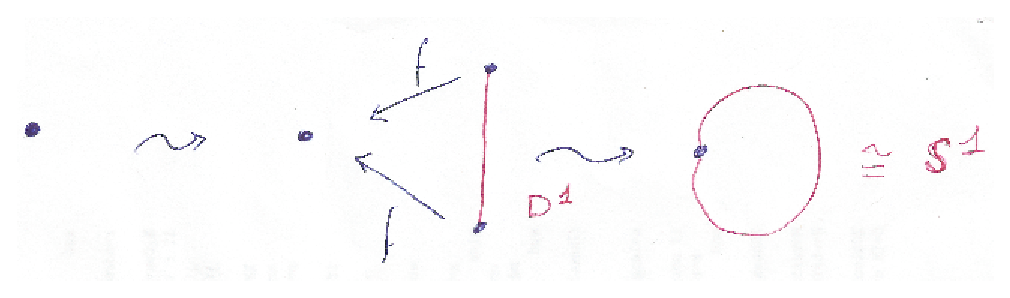
\includegraphics[scale=0.8]{Figures/CWej1}
\caption{\label{CWej1}$S^1$ construido como espacio de adjunción}
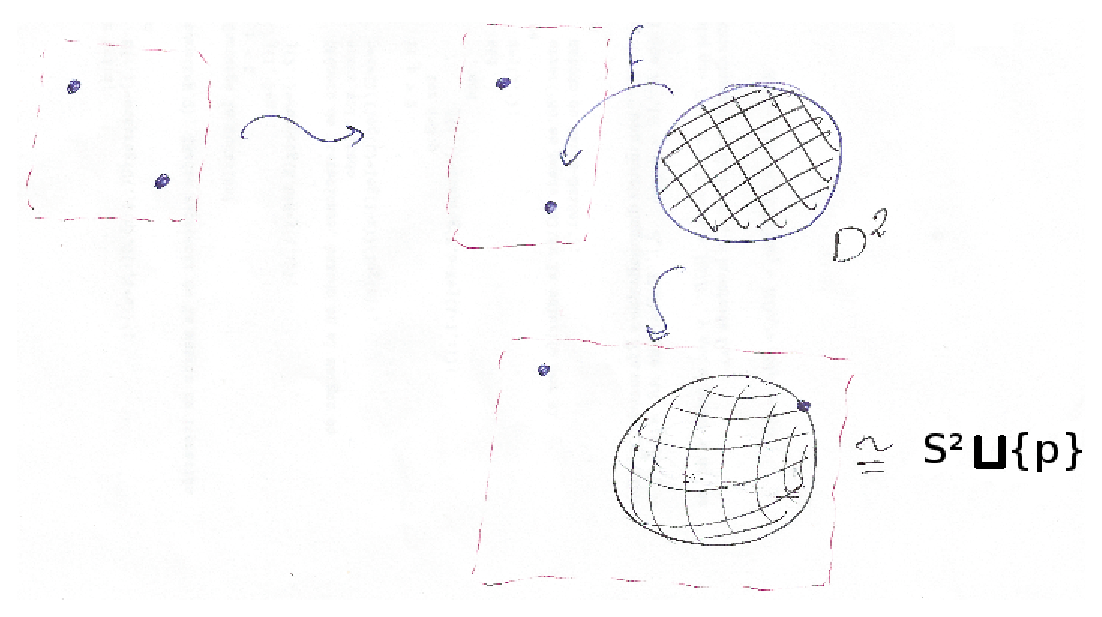
\includegraphics[scale=0.75]{Figures/CWej4}
\caption{\label{CWej4}$S^2$ construido como espacio de adjunción}
\end{figure}
\end{ejem}

\newpage
\subsection{Células y adjunción}
\cuadro{Supongamos que $X=D^n$ para algún $n > 0$ y $A=S^{n-1}$. Decimos que el espacio $$Y_f:=D^n\cup_f Y$$ es la \textbf{adjunción de una $n$-célula} al espacio $Y$.}

\begin{ejem}
En las figuras \ref{CWej1} y \ref{CWej4}, vemos cómo $S^1\cong \star_f$ y $S^2 \cong (\star\sqcup\star)_f$, siendo $\star$ un espacio puntual arbitrario. En general, el ejemplo \ref{Sn_CW} nos describe cómo expresar $S^n$ como adjunción de una célula a un espacio puntual.
\end{ejem}

\begin{lema}\label{EntornoCompacto}
Sea $f: S^{n-1} \longrightarrow Y$ una aplicación continua. Si $Y$ es un compacto de Hausdorff, existe un entorno compacto $U_f$ de $Y$ en $Y_f$ tal que $Y$ es un RDF de $U_f$.
\end{lema}

\begin{proof}
Sea $U=\{x \in D^n: \|x\| \geq 1/2\}$. $U$ es un entorno compacto de $S^{n-1}$ en $D^n$.
\\

Se define la homotopía $F: (U \sqcup Y)\times I \longrightarrow U\sqcup Y$ como $$F(x,t)=\begin{cases}x &\mbox{ si }x \in Y \\(1-t)x+t\frac{x}{\|x\|} &\mbox{ si }x \in U\end{cases}$$ Se tiene que $F$ es una aplicación continua y verifica que
\begin{enumerate}
\item $F(x,0)=x$ para todo $x \in U\sqcup Y$.
\item $F(x,1) \in S^{n-1}\sqcup Y$ para todo $x \in U \sqcup Y$.
\item $F(x,t)=x$ para todo $x \in S^{n-1}\sqcup Y$ y todo $t \in I$.
\end{enumerate}
Se sigue que $S^{n-1}\sqcup Y$ es un retracto por deformación fuerte de $U\sqcup Y$.
\\

Si $\pi: D^n \sqcup Y \longrightarrow Y_f$ denota a la aplicación cociente, se define $U_f$ como la imagen de $U$ mediante $\pi$. Queremos ver que $Y$ es un retracto por deformación fuerte de $U_f$ en $Y_f$.Para ello, considérese la homotopía $$\funcio{G}{U_f\times I}{U_f}{([x],t)}{[F(x,t)]}$$

Es fácil ver que $G$ está bien definida. Para ver que es continua, considérese el diagrama conmutativo
$$\begin{array}{ccccc}
&(U\sqcup Y)\times I&\xrightarrow{F}	& U\sqcup Y&\\
\pi\times 1_I&\downarrow			 & \circlearrowleft	& \downarrow&\pi\\
&U_f\times I & \xrightarrow{G}&U_f&
\end{array}$$

Dado que $F$ y $\pi$ son continuas, se tiene que $G\times (\pi\times 1_I)=\pi\circ F$ es continua. Dado que $U_f\times I$ tiene la topología producto y $U_f$ es un espacio cociente, se sigue que $G$ es continua. De aquí se sigue que $Y$ es un retracto por deformación fuerte de $U_f$.
\end{proof}

\begin{prop}Dada una aplicación continua $f: S^{n-1} \longrightarrow Y$, $$H_p(Y_f,Y)\cong\begin{cases}\mb{Z} & \mbox{ si }p=n \\ 0 & \mbox{ si no}\end{cases}$$\end{prop}

\begin{proof}Consideremos la composición $$h: D^n \hookrightarrow D^n\sqcup Y \xrightarrow{\pi} Y_f$$  $D^n-S^{n-1}$ es homeomorfo a $Y_f-Y$, puesto que $Y_f=Y\cup_f D^n$, de forma que $h$ induce un homeomorfismo relativo entre los pares $(D^n,S^{n-1})$ e $(Y_f,Y)$.
\\

$S^{n-1}$ es un RDF del entorno compacto $U=\{x \in D^n: \|x\| \geq 1/2\}$, y sabemos por el lema \ref{EntornoCompacto} que $Y$ es un RDF de algún entorno $U_f$ compacto de $Y$ en $Y_f$. Por el teorema del homeomorfismo relativo, se tiene que $$h_*: H_*(D^n,S^{n-1}) \longrightarrow H_*(Y_f,Y)$$ es un isomorfismo.
\\

Se tiene entonces que $$H_*(Y_f,Y) \cong H_*(D^n,S^{n-1}) \cong \tilde{H}_*(S^n)\cong\begin{cases}\mb{Z} & \mbox{ si }p=n \\ 0 & \mbox{ si no}\end{cases}$$\end{proof}

\newpage
\begin{prop}\cuadro{\label{HomoCW} Sea $Y$ un espacio topológico y $f: S^{n-1} \longrightarrow Y$ una aplicación continua. Si $$f_*: \tilde{H}_{n-1}(S^{n-1}) \longrightarrow H_{n-1}(Y)$$ se tiene que
\begin{enumerate}
\item $H_p(Y_f)\cong H_p(Y)$ para todo $p$ distinto a $n$ y $n-1$.
\item $H_{n-1}(Y_f)\cong H_{n-1}(Y)/\im f_*$
\item La siguiente sucesión es exacta: $$0 \longrightarrow H_n(Y) \longrightarrow H_n(Y_f) \longrightarrow \ker f_* \longrightarrow 0$$
\end{enumerate}}
\end{prop}

\begin{proof}
Consideremos la sucesión exacta larga asociada al par de espacios $(Y_f,Y)$: $$H_{p+1}(Y_f,Y) \longrightarrow H_p(Y) \xrightarrow{\beta} H_p(Y_f) \longrightarrow H_p(Y_f,Y)$$ Como vimos en el ejemplo \ref{Sn_CW}, se tiene que $$H_p(Y_f,Y)\cong \tilde{H}_p(S^n) \cong \tilde{H}_{p-1}(S^{n-1})$$

Para $p\neq n,n-1$, se tiene que $\tilde{H}_p(S^n)=0$, por lo que $\ker \beta=0$ y $\im \beta=H_p(Y_f)$. Se sigue entonces la primera afirmación: $$H_p(Y_f) \cong H_p(Y)$$

Para $p=n$ y $p=n-1$, se tiene la sucesión exacta \begin{multline*}
0=\tilde{H}_n(S^{n-1}) \longrightarrow H_n(Y) \longrightarrow H_n(Y_f) \xrightarrow{\beta} \tilde{H}_{n-1}(S^{n-1}) \xrightarrow{f_*} \\ \xrightarrow{f_*} H_{n-1}(Y) \xrightarrow{\alpha} H_{n-1}(Y_f)\longrightarrow \tilde{H}_{n-2}(S^{n-1})=0
\end{multline*}
donde $\im \beta=\ker f_*$, $\im f_*=\ker \alpha$ y $\im \alpha=H_{n-1}(Y_f)$ por exactitud. Aplicando el primer teorema de isomorfia, se tiene la segunda afirmación: $$H_{n-1}(Y_f)=\im \alpha \cong \frac{H_{n-1}(Y)}{\ker \alpha}=\frac{H_{n-1}(Y)}{\im f_*}$$

Ahora bien: como $\im \beta=\ker f_*$, la sucesión $$0 \longrightarrow H_n(Y) \longrightarrow H_n(Y_f) \xrightarrow{\beta} \ker f_* \longrightarrow 0$$ es exacta, que es la tercera afirmación.
\end{proof}

\section{Espacios CW-complejos}
Sean $D_1^n,\dots, D_p^n$ una cantidad finita de $n$-células disjuntas con respectivas fronteras $S^{n-1}_1,\dots,S^{n-1}_p$. Dado un $1 \leq i \leq p$, considérese la aplicación continua $$f_i: S^{n-1}_i \longrightarrow Y$$ siendo $Y$ un espacio topológico arbitrario. Definimos sobre $D^n_1\sqcup \dots \sqcup D^n_p\sqcup Y$ la siguiente relación de equivalencia: $$\forall x_i \in S^{n-1}_i \quad x_i \sim f_i(x_i)$$ y se define entonces $$Y_{f_1,\dots,f_p}=\frac{D^n_1\sqcup \dots \sqcup D^n_p\sqcup Y}{\sim}$$

\begin{prop} Sea $(X,Y)$ un par de espacios compactos de Hausdorff. Si existe un homeomorfismo relativo $$F: (D^n_1\sqcup \dots \sqcup D^n_p, S^{n-1}_1\sqcup \dots \sqcup S^{n-1}_p) \longrightarrow (X,Y)$$ que sea una prolongación continua de $f_1,\dots,f_p$, entonces $X$ es homeomorfo a $Y_{f_1,\dots,f_p}$.\end{prop}

\cuadro{\lista{\item Un \textbf{CW-complejo finito de dimensión 0 }es una colección finita de puntos $\{p_1,\dots,p_n\} \subset \mbR^t$. \item Sea $Y$ un CW-complejo finito de dimensión $k \geq 0$. Un \textbf{CW-complejo finito de dimensión $k+1$} es un espacio topológico $C_2$ que puede expresarse como adjunción de una cantidad finita de $(k+1)$-células a $Y$.}}

\begin{ejem} $S^n$ admite estructura de CW-complejo, siguiendo el ejemplo \ref{Sn_CW}. Veamos un par de ejemplos adicionales:\end{ejem}

\begin{figure}[h]
\centering
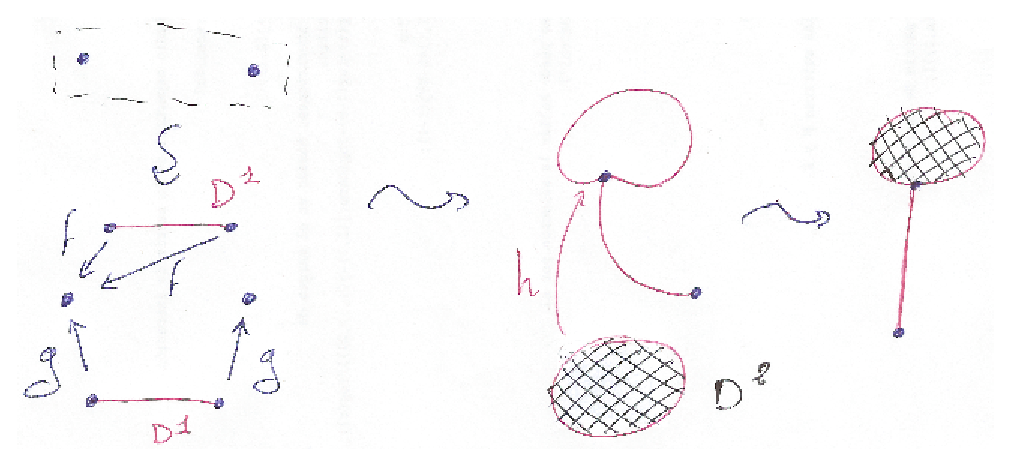
\includegraphics[scale=0.7]{Figures/CWej2}
\caption{Los postes de tráfico y las guindas admiten estructura de CW-complejo.}
\end{figure}

\begin{figure}[h]
\centering
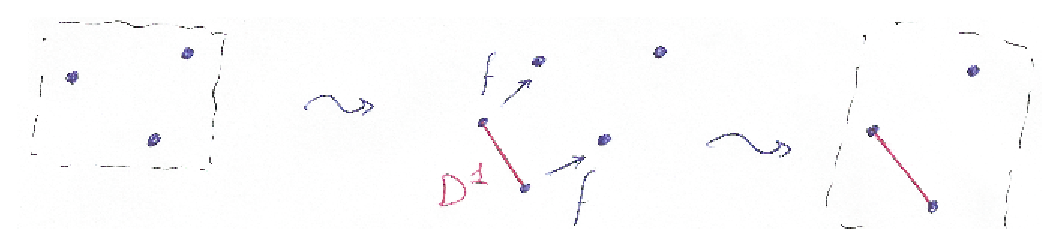
\includegraphics[scale=0.7]{Figures/CWej3}
\caption{El borde de una célula de dimensión 1 o superior siempre tiene que adherirse a algo, pero es admisible que queden 0-células (puntos) libres.}
\end{figure}

\newpage
Hemos definido los CW-complejos de dimensión $n$ como un proceso iterativo que da lugar a una serie de CW-complejos intermedios $$X^0 \subseteq X^1 \subseteq \dots \subseteq X^n$$ Cada uno de los $X^k$ se denomina \textbf{$k$-esqueleto} del CW-complejo. Notar que $X^n$ es el CW-complejo completo.

\begin{ejem} El ejemplo \ref{Sn_CW} describe una construcción de $S^2$ como CW-complejo de forma que el 1-esqueleto y el 0-esqueleto son el mismo conjunto, porque no adjuntamos ninguna 1-célula a $X^0$. Pero un CW-complejo puede admitir muchas estructuras diferentes. 
\\

Consideremos la siguiente estructura: sea $X^0=\{(1,0,0), (0,1,0), (-1,0,0)\}$, tres puntos del ecuador. Adjuntamos a $X^0$ tres 1-células, $e^1_1$, $e^1_2$ y $e^1_3$, de forma que $S^1\cong X^1$.

\begin{figure}[h]
\centering
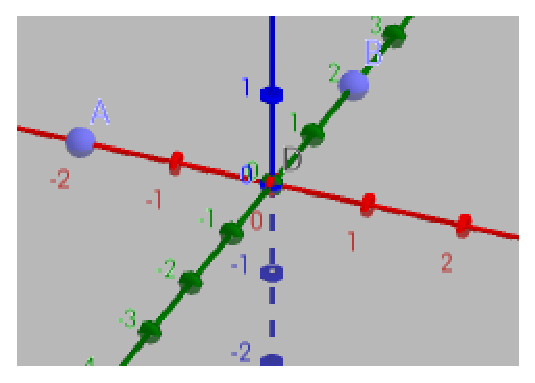
\includegraphics[scale=0.71]{Figures/S2paso1}
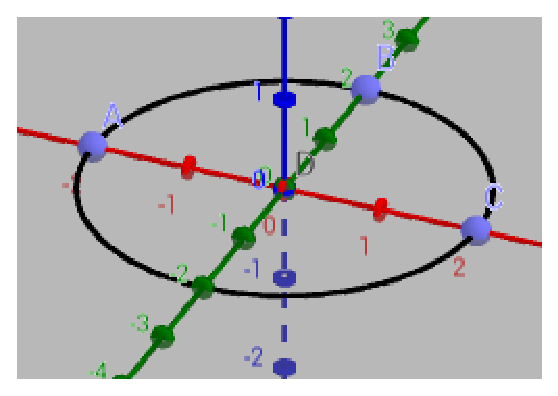
\includegraphics[scale=0.7]{Figures/S2paso2}
\end{figure}

\newpage
Finalmente, adjuntamos dos 2-células $e^2_1$ y $e^2_2$ a $X^1$. Esto sería $X^2$, que es homeomorfo a todo $S^2$.

\begin{figure}[h]
\centering
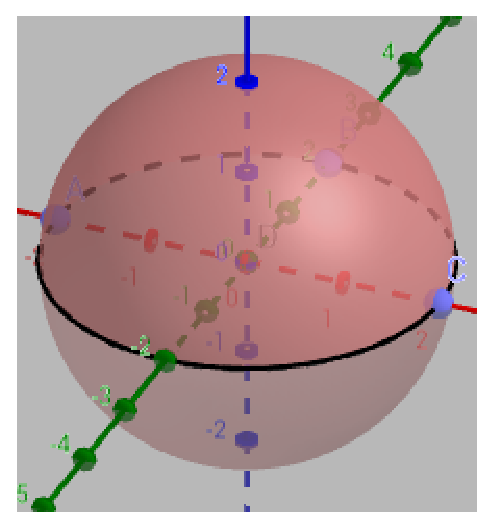
\includegraphics[scale=0.7]{Figures/S2paso3}
\end{figure}

En general, podemos generar una descomposición de $S^n$ de forma que cada $k$-esqueleto sea $S^k$ ($k=0,1,2,\dots,n$); no obstante, en ese caso tendríamos que el 0-esqueleto son dos puntos, dado que \[S^0=\{x \in D^1: \|x\|=1\}=\{x \in [-1,1]: |x|=1\}=\{\pm 1\}\]
\end{ejem}

De esta forma, tenemos que un espacio topológico no induce una descomposición como CW-complejo de forma única. Si comparamos este proceso con el que seguimos en el ejemplo \ref{Sn_CW}, tenemos que no tienen el mismo número de células y sus 1-esqueletos no son homeomorfos, de forma que no son \textit{estructuras equivalentes}.
\newpage

\begin{teo}[Caracterización de CW-complejos finitos]\label{TCCWF}\cuadro{Un espacio topológico compacto $X$ es un CW-complejo finito de dimensión $n$ si y sólo si podemos hallar una sucesión de subespacios $$X^0 \subseteq X^1 \subseteq \dots \subseteq X^n=X$$ y una partición de subconjuntos $$\{e_i^k:\; k=0,1,\dots,n; \;i=1,2,\dots,r_k\}$$ (llamada \textbf{descomposición celular}) tales que \lista{\item Existe un homeomorfismo relativo $h: (D^k,S^{k-1}) \longrightarrow (\overline{e}^k_i,\overline{e}^k_i-e^k_i)$ para cada $i$ y $k$. \item Dado un $1 \leq k \leq n$, $\overline{e}^k_i-e^k_i \subseteq X^{k-1}$.}}\end{teo}

Hagamos un par de incisos en este teorema.

\begin{enumerate}
\item Observar que $\overline{e^k_i}-(\overline{e^k_i}-e^k_i)=e^k_i$. Aplicando la condición 1 del teorema anterior, se sigue que $e^k_i$ es homeomorfo a una bola abierta de $\mbR^k$. Esto implica que las $n$-células son conexas, compactas y abiertas para todo $n > 0$.

\item La condición de compacidad viene dada porque la adjunción de espacios compactos es compacto, pero ninguna de las otras condiciones garantizan que $X$ sea compacto.
\end{enumerate}

\begin{ejem}
\begin{enumerate}
\item Este teorema proporciona otra forma de ver que $S^n$ admite una estructura de CW-complejo, pero nos ceñiremos al caso $n=1$ por simplicidad.
\\

Sea $f: [0,2\pi] \longrightarrow \mb{C}$ la función $f(t)=e^{it}$. Se tiene que $S^1$ admite una estructura de CW-complejo tomando los esqueletos $X^0=\{f(0)\}$ y $X^1=S^1$, y la descomposición celular dada por $$\{\{f(0)\},f(]0,1[)\}$$

\item El segmento $I$ admite una estructura de CW-complejo dada por la descomposición celular $$\{\{0\},\{1\},]0,1[\}$$

\item En general, toda línea poligonal formada por una cantidad finita de segmentos admite una estructura trivial de CW-complejo.
\end{enumerate}
\end{ejem}

\begin{figure}[h]
\centering
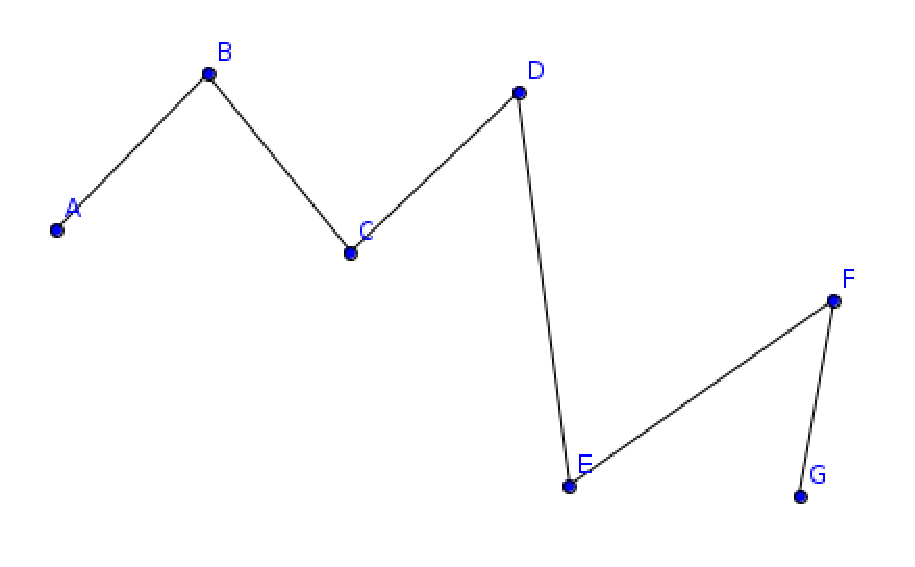
\includegraphics[scale=0.8]{Figures/Poligonal.eps}
\caption{Los puntos $A,B,\dots,G$ conforman el 0-esqueleto de la línea poligonal.}
\end{figure}

\begin{ejem}
\begin{enumerate}
\item El conjunto $A=\{1/n: n \in \mb{N}\}\cup \{0\}$ con la topología inducida por la métrica usual de $\mbR$ no es un CW-complejo finito, porque no es compacto.

\item El \textbf{pendiente hawaiiano} es un ejemplo de espacio topológico compacto que no tiene estructura de CW-complejo. Si $C(\alpha,\beta)$ denota la circunferencia de centro $\alpha \in \mbR^2$ y radio $\beta > 0$, se definen los pendientes hawaiianos como el espacio topológico $$H=\bigcup_{n=1}^\infty C(\alpha_n,\beta_n); \quad \alpha_n=\left(\frac{1}{n},0\right); \quad \beta_n=\frac{1}{n}$$ Intuitivamente, esto se debe a que tiene una cantidad infinita de anillos, y cada uno tendría que ser una 1-célula independiente.
\end{enumerate}
\end{ejem}

\begin{figure}[h]
\centering
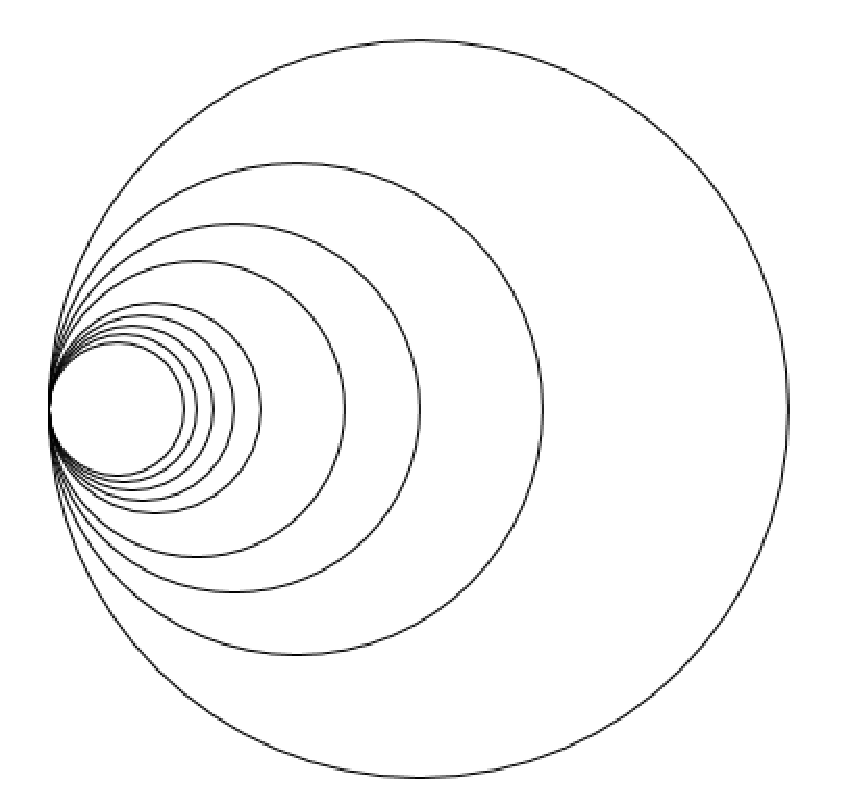
\includegraphics[scale=0.6]{Figures/Hawaii.eps}
\caption{Primeras iteraciones del pendiente hawaiiano}
\end{figure}

\begin{prop}\label{CWProd} El producto de CW-complejos finitos es un CW-complejo finito.\end{prop}

\begin{proof}
Sea $C=\{e_i^k:\; k=0,1,\dots,n; \;i=1,2,\dots,r_k\}$ una descomposición celular de $X$ y $D=\{f_\ell^j:\; j=0,1,\dots,m; \;\ell=1,2,\dots,r_j\}$ una descomposición celular de $Y$. Queremos ver que el conjunto $$E=\{u\times v: u\in C, v\in D\}$$ forma una descomposición celular de $X\times Y$.
\\

Claramente, los elementos de $E$ son disjuntos dos a dos por construcción. Veamos que forman un recubrimiento de $X\times Y$: $$X\times Y=\left(\bigcup_{u \in C}u\right)\times\left(\bigcup_{v \in D}v\right)=\bigcup_{\substack{u \in C\\v \in D}}u\times v$$

Veamos la \textbf{condición 1} del teorema \ref{TCCWF}: dados $i,j,k,\ell$, \begin{multline*}
U=\overline{e^k_i\times f^\ell_j}-e^k_i\times f^\ell_j=\overline{e}^k_i\times \overline{f}^\ell_j-e^k_i\times f^\ell_j=\\=[(\overline{e}^k_i-e^k_i)\times \overline{f}^\ell_j]\cup[\overline{e}^k_i\times (\overline{f}^\ell_j-f^\ell_j)] \end{multline*} Sabemos por hipótesis que $(\overline{e}^k_i-e^k_i) \subseteq X^{k-1}$ y $\overline{f}^\ell_j-f^\ell_j \subseteq Y^{\ell-1}$, por lo que $U \subseteq (X\times Y)^{k+\ell-1}$.
\\

Pasemos a la \textbf{condición 2}: sean $u \in C$ y $v \in D$. Si $$f: (D^k,S^{k-1}) \longrightarrow (\overline{u},\overline{u}-u); \quad g: (D^\ell,S^{\ell-1}) \longrightarrow (\overline{v},\overline{v}-v)$$ son homeomorfismos relativos, se tiene que $$f\times g: (D^{k+\ell},S^{k+\ell-1}) \longrightarrow (\overline{u\times v},\overline{u\times v}-u\times v)$$ es un homeomorfismo relativo.\end{proof}

\begin{ejem}\label{CWlindro}
\begin{enumerate}
\item El cilindro con bordes se define como la variedad $C=S^1\times [0,1]$. Podemos asignar una estructura de CW-complejo a $C$ usando una estructura prefijada de $S^1$ y otra de $[0,1]$:

\[[0,1] \begin{cases}
\mbox{0-células:}&p=\{0\}, q=\{1\}\\
\mbox{1-células:}&\alpha=]0,1[
\end{cases} \quad
S^1 \begin{cases}
\mbox{0-células:}&r=\{(1,0)\}\\
\mbox{1-células:}&\beta=S^1-r
\end{cases}\]

Estas estructuras inducen la siguiente descomposición celular sobre el cilindro:

\[C \begin{cases}
\mbox{0-células:}&p\times r,\, q\times r\\
\mbox{1-células:}&\alpha \times r,\, p\times \beta,\, q\times \beta\\
\mbox{2-células:}&\alpha \times \beta
\end{cases}\]

\begin{figure}[h]
\centering
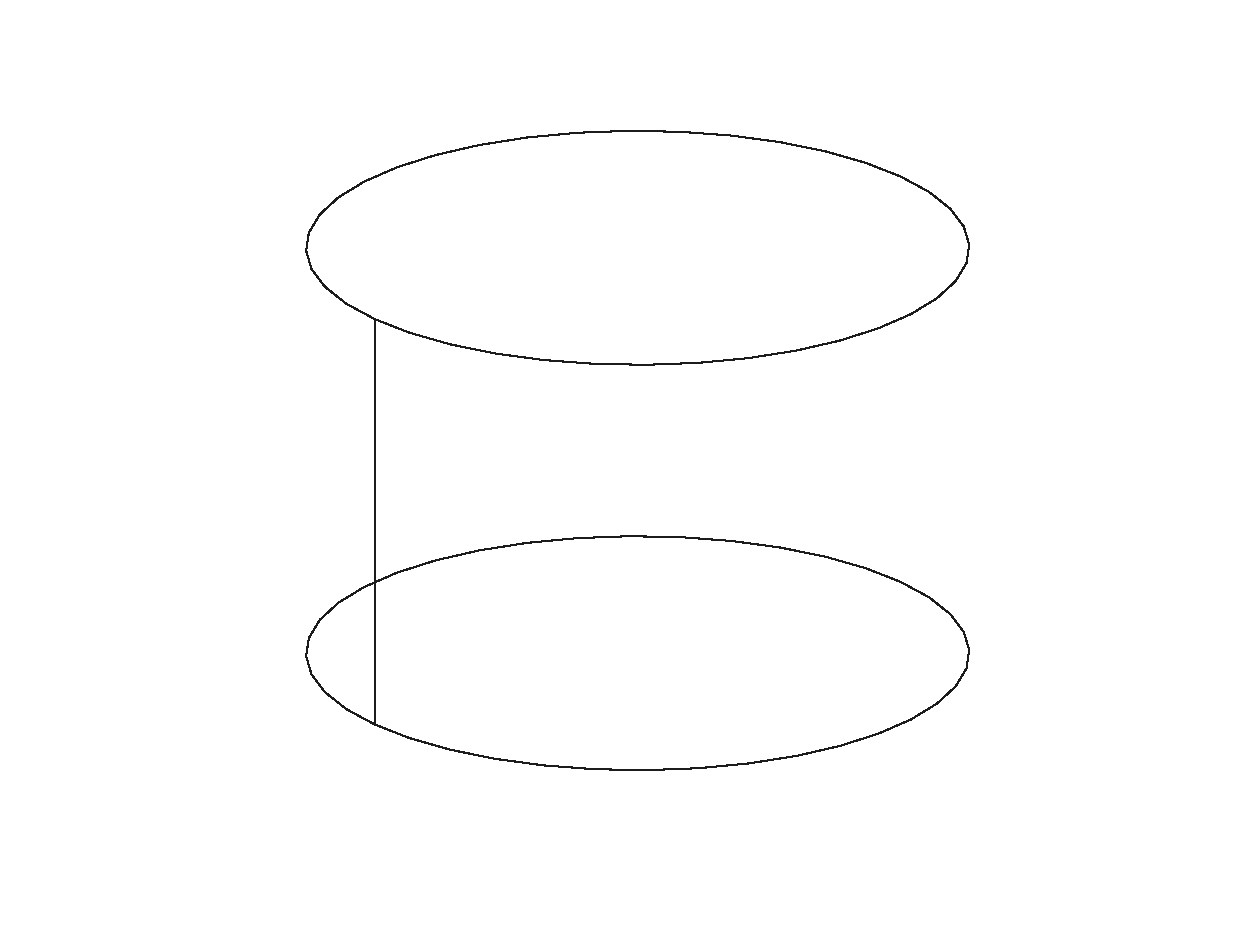
\includegraphics[scale=0.4]{Figures/1EsqCilindro.eps}
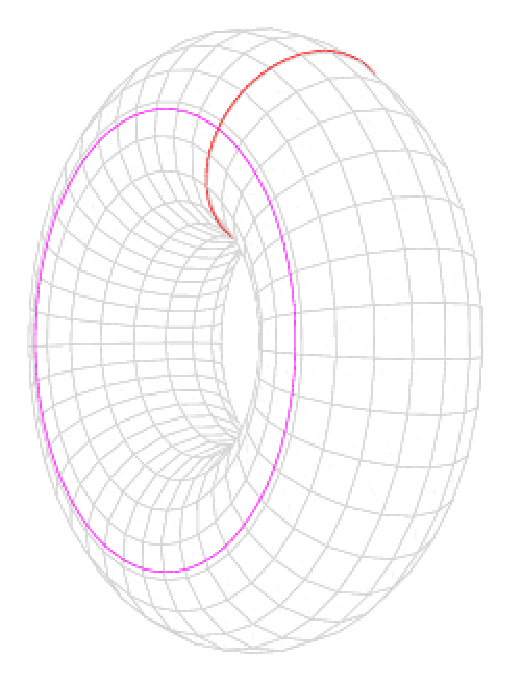
\includegraphics[scale=0.5]{Figures/FiguraOcho.eps}
\caption{Izquierda: 1-esqueleto del cilindro. Derecha: 1-esqueleto del toro, que es una figura ocho. Observar que el 1-esqueleto del cilindro se puede retraer en una figura ocho.}
\end{figure}

\item El \textbf{toro de Clifford} se define como la variedad $S^1\times S^1$, que es homeomorfa al toro llano y al toro paramétrico.\\

Consideremos la siguiente descomposición celular de $S^1$: \[S^1 \begin{cases}
\mbox{0-células:}&p=\{(1,0)\}\\
\mbox{1-células:}&\alpha=S^1-p
\end{cases} \quad
S^1 \begin{cases}
\mbox{0-células:}&r=\{(1,0)\}\\
\mbox{1-células:}&\beta=S^1-r
\end{cases}\]

Estas estructuras inducen la siguiente descomposición celular sobre el toro de Clifford:
\[S^1\times S^1 \begin{cases}
\mbox{0-células:}&p\times r\\
\mbox{1-células:}&\alpha \times r,\, p\times \beta\\
\mbox{2-células:}&\alpha \times \beta
\end{cases}\]
\end{enumerate}
\end{ejem}

\subsection{Subcomplejos}
\cuadro{Sea $X$ un CW-complejo finito y $C(X)$ una descomposición celular de $X$. Decimos que un subespacio $A \subseteq X$ es un \textbf{subcomplejo} de $X$ si $A$ \textit{absorbe} todas las células de $X$ que toca: $$\forall e \in C(X) \quad e\cap A\neq \emptyset \implies \overline{e} \subseteq A$$}

Todo subcomplejo de un cierto complejo $X$ conforma un subespacio cerrado. Además, aplicando el teorema de caracterización de CW-complejos finitos, se tiene que todo subcomplejo es un complejo en sí mismo.
\\

En particular, todos los $k$-esqueletos de $X$ son subcomplejos.

\begin{prop}Si $A$ es un subcomplejo de un CW-complejo finito $X$, $A$ es un RDF de algún entorno compacto de $A$ en $X$.\end{prop}

\begin{proof}
Sea $N$ el número de células que componen el espacio $X-A$. Si $N=0$, $X=A$, por lo que $A$ es un RDF de $X$ de forma trivial y se sigue la tesis por compacidad de $X$. Si $N=1$, existe una aplicación $f: S^{n-1} \longrightarrow A$ continua tal que $$X=A\cup_f D^n$$ En tal caso, podemos limitarnos a aplicar el lema \ref{EntornoCompacto}.
\\

Supongamos que el resultado es cierto para cualquier par de CW-complejos finitos $(Y,B)$ tales que $Y-B$ posee a lo sumo $N-1$ células, y sea $(X,A)$ un par de CW-complejos tales que $X-A$ tiene exactamente $N$ células. Si $e^m_i$ es una célula de $X-A$ de dimensión máxima, se define el subespacio $$Y=X-e^m_j$$

\noindent\textbf{Paso 1: $A$ es un RDF de un entorno compacto de $A$ en $Y$}
\\
Queremos ver que $Y$ es un subcomplejo de $X$. Como $e^m_i$ es una célula de dimensión máxima, todas las células de $X-A$ tienen dimensión $m$ o menos; de esta forma, toda célula de $X$ con dimensión mayor que $m$ forma parte del subcomplejo $A$. En consecuencia, si $e^k_j$ es una célula de $Y$, se tiene que $e^k_j \subset A$ ó $k \leq m$.
\\

Si $e^k_j \subset A$, $\overline{e^k_j} \subseteq A$ por ser $A$ un subcomplejo de $X$, de forma que $$e^m_i \cap \partial e^k_j \subseteq e^m_i \cap A=\emptyset$$ En cambio, si $k \leq m$, se tiene en virtud del teorema de caracterización de CW-complejos finitos que $$\partial e^k_j=\overline{e^k_j}-e^k_j\subseteq X^{k-1}$$ Dado que $k-1 < m$, se cumple una vez más que $e^m_i \cap \partial e^k_j =\emptyset$.  Se sigue que $Y$ es subcomplejo de $X$.
\\

Dado que $A$ es un subcomplejo de $X$ y $e^m_i \subset X-A$, $A\cap e^m_i=\emptyset$, por lo que es un subcomplejo de $Y$. Como $Y$ tiene una célula menos que $X$, el par $(Y,A)$ verifica la hipótesis de inducción, por lo que existe un entorno $U_1$ compacto de $A$ en $X$ tal que $A$ es un RDF de $U_1$.
\\

\noindent\textbf{Paso 2: Construcción del entorno compacto buscado}
\\
Sea $f: S^{m-1} \longrightarrow Y$ una aplicación continua tal que $X=Y\cup_f D^m$. Podemos hallar un homeomorfismo relativo $$\phi: (D^m,S^{m-1}) \longrightarrow (\overline{e^m_i}, \overline{e^m_i}-e^m_i)$$ que extienda a $f$ de forma continua. Como $U_1$ es compacto en $Y$ y $\phi$ es un homeomorfismo, se tiene que $\phi^{-1}(U_1)$ es un compacto de $S^{m-1} \subset D^m$. Si $$\funcio{r}{D^m-\{0\}}{S^{m-1}}{x}{\frac{x}{\|x\|}}$$ es la retracción radial, se tiene que $$V=\{\phi(x): x \in D^m,\; \|x\| \geq 1/2\; \land\; r(x) \in \phi^{-1}(U_1)\}$$ también es compacto.
\\

Veamos cómo se construye el conjunto $V$: las células se adhieren al CW-complejo por el borde, por lo que podemos pensar que la aplicación $\phi$ abomba $D^m$ para darle forma de hemisferio y pegarlo a $Y$ por la línea del ecuador. Se tiene entonces que $X=Y\cup \phi(D^m)$, como podemos ver en la figura \ref{ECompacto1}. 
\\

Dado que $Y\cap \phi(D^m)=f(S^{m-1})$, $\phi^{-1}(U_1)=f^{-1}(U_1)$ está contenido en $S^{m-1}$. Por tanto, $x$ no tiene por qué estar en $\phi^{-1}(U_1)$, por lo que lo retraemos mediante una aplicación adicional. Finalmente, elegimos sólo los puntos que están entre las esferas concéntricas de radios $1/2$ y $1$, por lo que $\phi^{-1}(V)$ tendrá el aspecto de la figura \ref{PhiMenos1V}.
\\

\begin{figure}[h]
\centering
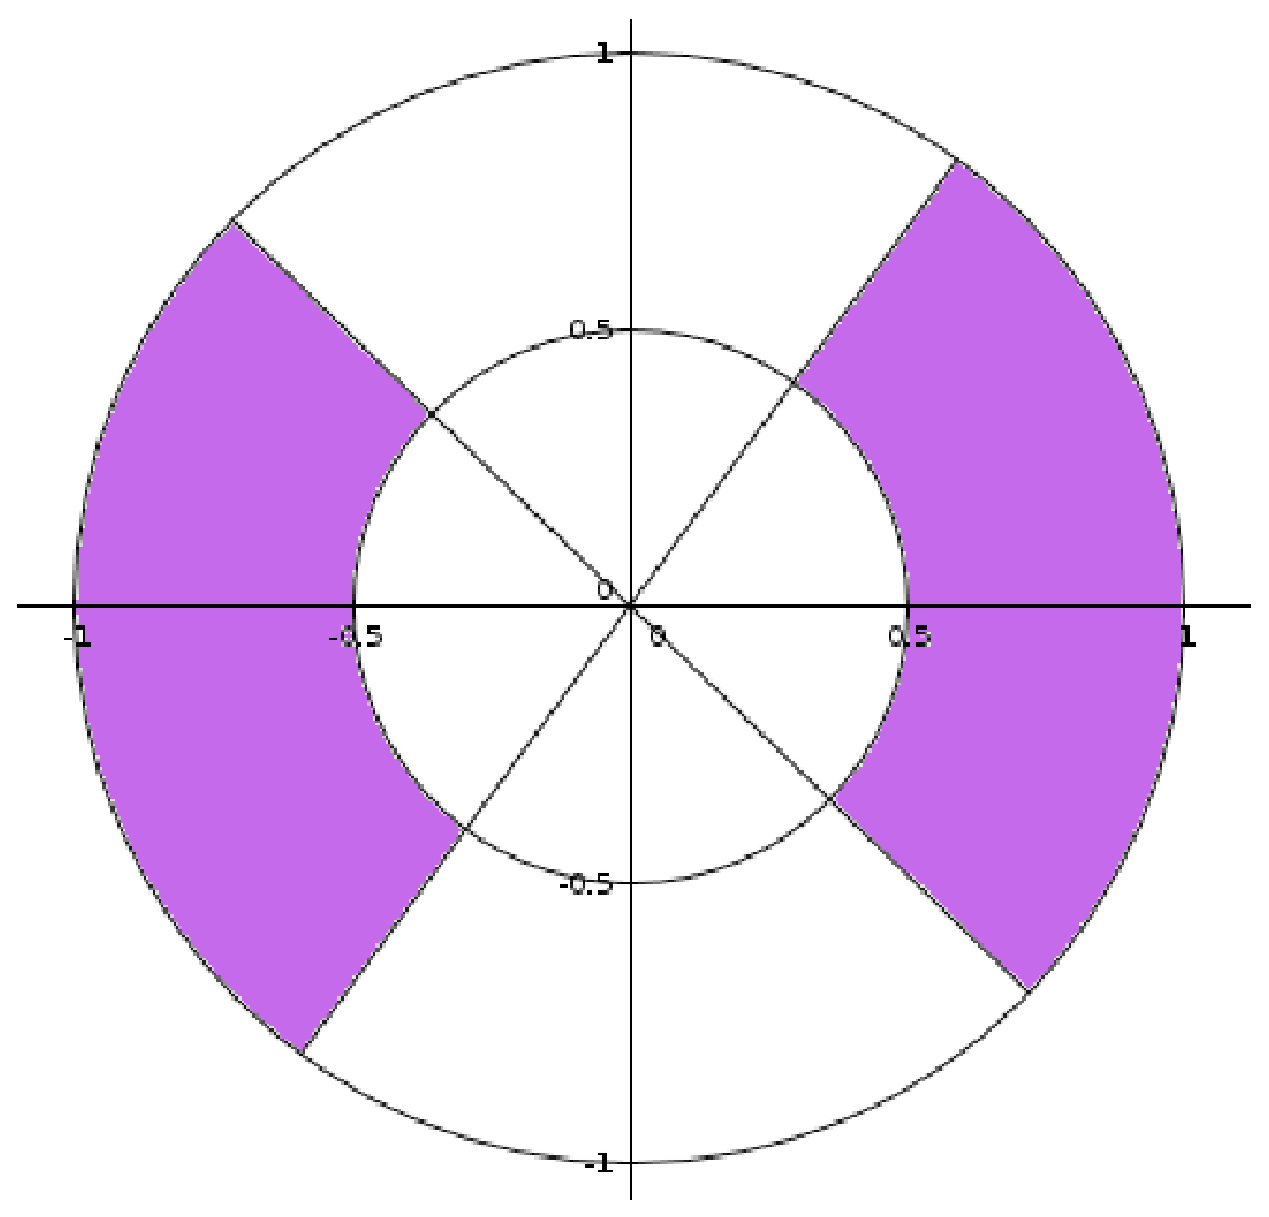
\includegraphics[scale=0.4]{Figures/PhiMenos1V}
\caption{\label{PhiMenos1V} El conjunto $\phi^{-1}(V)$ corresponde a la región violeta. $\phi^{-1}(U_1)$ son los puntos de la región violeta que recaen sobre la esfera de radio 1.}
\end{figure}

$U_1 \cap V$ es un retracto por deformación de $V$ y $A$ es un retracto por deformación de $U_1$, de forma que $A$ será un retracto por deformación de $U_1 \cup V$ componiendo ambas retracciones. Dicha retracción se ilustra en la figura \ref{ECompacto1}.
\\

\begin{figure}[h]
\centering
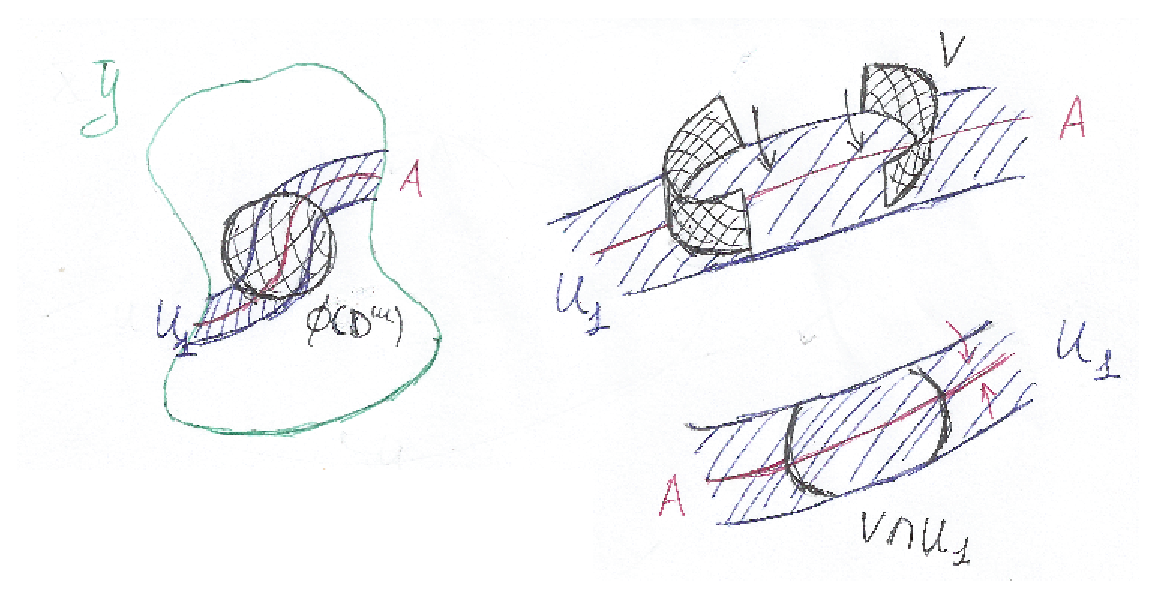
\includegraphics[scale=0.75]{Figures/ECompacto1}
\caption{\label{ECompacto1} Izquierda: situación del paso 2. Derecha: descripción gráfica de cómo $U_1\cup V$ se retraería en $A$.}
\end{figure}

\noindent\textbf{Paso 3: $U_1\cup V$ es un entorno compacto de $A$}
\\
Ya sabemos que $U_1 \cup V$ se puede retraer en $A$. Dado que es unión de compactos, es trivialmente compacto, de forma que habremos terminado la demostración si podemos probar que $U_1 \cup V$ es entorno en $X$ de $A$.
\\

Sea $y \in \mbox{int}_Y(U_1)$. Si $y \not\in V$, $y \in \mbox{int}_X(U_1)$ (repersentado como una banda en la ilustración \ref{ECompacto2}), por lo que también estará en $\mbox{int}_X(U_1 \cup V)$.
\\

\begin{figure}[h]
\centering
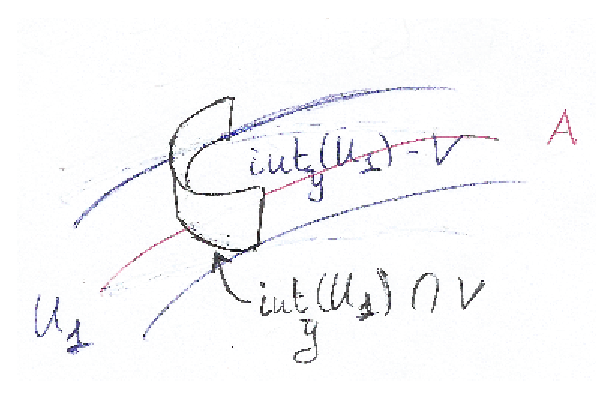
\includegraphics[scale=1]{Figures/ECompacto2}
\caption{\label{ECompacto2} El interior de $U_1$ en $Y$. $V$ es el medio cilindro ortogonal a la cinta.}
\end{figure}

Si $y \in V$, se tiene que $y \in \overline{e^m_i}-e^m_i=\phi(D^m-\partial D^m)=f(S^{m-1})$. $\phi^{-1}(\mbox{int}_Y(U_1))$ es un abierto de $S^{m-1}$, que contiene a $\phi^{-1}(y)$ (por cómo se define $V$), de forma que $$\phi^{-1}(y) \in \mbox{int}_{S^{m-1}}\phi^{-1}(V) \implies y \in \mbox{int}_{\overline{e^m_i}}(V)$$ Dado que $e^m_i$ es una célula de $X$, se sigue que $y \in \mbox{int}_X(U_1\cup V)$. 
\\

Como $U_1$ es un entorno de $A$ en $Y$, $$A \subseteq \mbox{int}_Y(U_1)\subseteq \mbox{int}_X(U_1\cup V)$$ por lo que $U_1\cup V$ es entorno de $A$ en $X$. Pero eso es lo que nos quedaba por demostrar. 
\end{proof}

\subsection{Grupos de homología celular}
\begin{teo} Dado un $n \geq 1$,
\[H_p(S^n)\cong \begin{cases}\mb{Z} & \mbox{ si }p=0,n \\ 0 & \mbox{ si no}\end{cases} \quad\land \quad \tilde{H}_p(S^n)\cong \begin{cases}\mb{Z} & \mbox{ si }p=n \\ 0 & \mbox{ si no}\end{cases}\]
\end{teo}

\begin{proof}
Como sabemos por el ejemplo \ref{RedSn}, $\tilde{H}_*(S^n)$ es isomorfo a $H_*(S^n,\star)$, siendo $\star$ el espacio puntual. Para $n=1$, se tiene que \[H_p(S^1,\star)\cong\frac{H_p(S^1)}{H_p(\star)}\cong \begin{cases}\mb{Z}&\mbox{ si }p=1\\0&\mbox{ si no}\end{cases}\]

Supongamos que existe un $n > 1$ tal que la tesis es cierta para $S^{n-1}$. Como sabemos por el ejemplo \ref{Sn_CW}, $S^n$ admite una estructura de CW-complejo dada por $$S^n\cong D^n\cup_f \star$$ siendo $f: S^{n-1} \longrightarrow \star$ la aplicación constante. La descomposición celular que induce esta estructura es $\{D^n,\star\}$.
\\

Utilizando la proposición \ref{HomoCW}, se tiene que \[H_p(S^n)\cong H_p(\star)=0 \quad \forall p\neq 0, n-1,n\]

$f$ induce un homomorfismo $f_*: \tilde{H}_{n-1}(S^{n-1}) \longrightarrow H_{n-1}(\star)$. Dado que $\star$ es convexo, se tiene que $H_{n-1}(\star)=0$, por lo que $\im f_*=0$. Se sigue que \[H_{n-1}(S^n)\cong \frac{H_{n-1}(\star)}{\im f_*}=\frac{0}{0}=0\] Además, en virtud del primer teorema de isomorfia, \[\ker f_*=\tilde{H}_{n-1}(S^{n-1})\cong \mb{Z}\]

Considérese la siguiente sucesión exacta: \[0 \longrightarrow H_n(\star) \xrightarrow{\alpha} H_n(S^n) \xrightarrow{\beta} \ker f_* \longrightarrow 0\] Dado que $H_n(\star)=0$, se tiene por exactitud que $\ker \beta=\im \alpha=0$ y $\im \beta=\ker f_*$, de forma que \[\beta: H_n(S^n) \xrightarrow{\quad\cong\quad}\ker f_* \cong \mb{Z}\] Por tanto, se tiene que \[H_p(S^n)\cong \begin{cases}\mb{Z}&\mbox{ si }p=0,n\\0&\mbox{ si no}\end{cases} \implies H_p(S^n,\star)=\frac{H_p(S^n)}{H_p(\star)}\cong \begin{cases}\mb{Z}&\mbox{ si }p=n\\0&\mbox{ si no}\end{cases}\]
\end{proof}

De aquí se sigue que los números de Betti de $S^n$ son $\beta_0(S^n)=1$, $\beta_n(S^n)=1$ y todos los demás cero, por lo que \[\chi(S^n)=\beta_0(S^n)+(-1)^n\beta_n(S^n)=1+(-1)^n=\begin{cases}2 &\mbox{ si }n=2k \\ 0 & \mbox{ si } n=2k+1\end{cases}\]

\begin{cor}\cuadro{Si $X$ es un CW-complejo finito y $X^k$ es el $k$-esqueleto de $X$, entonces $$H_j(X^k,X^{k-1})=0 \quad \forall j \neq k$$ Además, $H_k(X^k,X^{k-1})$ es un grupo abeliano libre con un generador por cada $k$-célula de $X$, conocido como el \textbf{grupo de homología celular} de orden $k$.}\end{cor}

\begin{proof}
Sabemos que $X^{k-1}$ es un subcomplejo de $X^k$. Por la proposición anterior, existe un entorno compacto $U \subseteq X^k$ de $X^{k-1}$ tal que $X^{k-1}$ es un retracto por deformación fuerte de $U$.
\\

Como $X$ es un CW-complejo finito, podemos hallar un homeomorfismo relativo $$\phi: (D_1^k\sqcup D_2^k\sqcup \dots \sqcup D^k_r, S_1^{k-1}\sqcup S_2^{k-1}\sqcup \dots \sqcup S^{k-1}_r) \longrightarrow (X^k,X^{k-1})$$ utilizando los homeomorfismos $h$ que nos proporciona el teorema de caracterización de CW-complejos finitos. Aplicando el teorema del homeomorfismo relativo, se sigue que 
\begin{multline*}
H_*(X^k,X^{k-1}) \cong H_*(D_1^k\sqcup D_2^k\sqcup \dots \sqcup D^k_r, S_1^{k-1}\sqcup S_2^{k-1}\sqcup \dots \sqcup S^{k-1}_r) \cong \\ \cong \sum^r_{i=1} H_*(D_i^k, S_i^{k-1}) \cong \sum^r_{i=1} \tilde{H}_*(S^k) \cong \tilde{H}_*(S^k)^r \cong \begin{cases}\mb{Z}^r&\mbox{ si }p=k\\0&\mbox{ si no}\end{cases}
\end{multline*}
\end{proof}

\begin{ejem}
Vamos a calcular la homología de la rosa de $p$ pétalos utilizando los grupos de homología celular. Por la proposición \ref{HomoCW}, tenemos que $$H_j(B_p)\cong H_j(\star)=0$$ para todo $j > 1$. Para $j=1$, tenemos que $$H_1(B_p)\cong \tilde{H}_1(B_p)\cong H_1(B_p,\star)$$ Dado que $\star$ es el 0-esqueleto de $B_p$, que tiene $p$ 1-células, se tiene que dicho grupo es isomorfo a $\mb{Z}^p$.
\end{ejem}

\subsection{Teorema del punto fijo de Brouwer}
Uno de los resultados clásicos de la topología algebraica es el \textbf{teorema del punto fijo de Brouwer}, de gran importancia en diversas áreas de la matemática tales como la teoría de juegos. La formulación estándar del teorema de Brouwer (así como la de otros muchos teoremas de punto fijo de análisis funcional) es la siguiente:

\begin{teo}[Teorema del punto fijo de Brouwer] Sea $f: D^n \longrightarrow D^n$ una función continua. Existe un $p \in D^n$ tal que $f(p)=p$.\end{teo}

\begin{proof}
Sea $f: D^n \longrightarrow D^n$ una aplicación continua. Supongamos que $f$ no posee puntos fijos; esto es, que $$\forall x \in D^n \quad f(x)\neq x \iff \|x-f(x)\| > 0$$ Consideramos entonces la semirrecta $$r_x=\{\mu u_x+x: \mu \geq 0\}; \quad u_x=\frac{x-f(x)}{\|x-f(x)\|}$$ que está bien definida. Se define la correspondencia $g: D^n \longrightarrow S^{n-1}$ que asigna a $x$ un punto $g(x)\in r_x\cap S^{n-1}$.
\\

\begin{figure}[h]
\centering
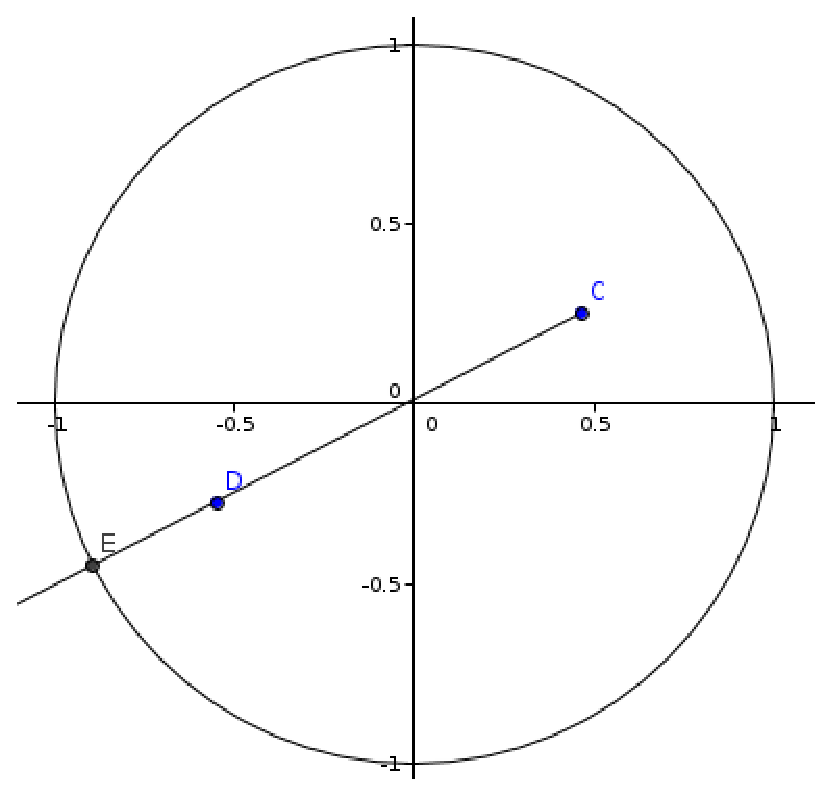
\includegraphics[scale=0.6]{Figures/Brouwer.eps}
\caption{La aplicación $g$ extiende una semirrecta que pasa por los puntos $C$ y $D=f(C)$ para tomar el punto de intersección con la esfera unidad. Dicho punto de intersección es $g(C)$. Intuitivamente, si $C \in S^{n-1}$, $g(C)$ es el propio $C$.}
\end{figure}

Queremos ver que $g(x)$ es un singulete. Dados dos puntos $p,q \in r_x$, existen $\lambda, \mu \geq 0$ tales que $$p=u_x\mu+x; \quad q=u_x\lambda+x \implies p-q=u_x(\mu-\lambda)$$ Tomando normas a ambos lados de la igualdad, \[\|p-q\|=|\mu-\lambda|\|u_x\|=|\mu-\lambda|\] de lo que se deduce que no hay dos puntos diferentes con la misma norma.
Por tanto, $g$ es una aplicación continua.
\\

Observar que, si $x \in S^{n-1}$, será el único punto de $r_x$ con norma 1. De aquí se sigue que $g$ fija los puntos de $S^{n-1}$, por lo que es un retracto fuerte e induce un epimorfismo $$g_*: H_n(D^n) \longrightarrow H_n(S^{n-1})$$

Como $D^n$ es convexo, $H_n(D^n)$ es un grupo trivial; no obstante, como acabamos de ver, $H_n(S^{n-1})$ tiene rango 1. Dado que $g_*$ es sobreyectiva, si llamamos $\alpha$ al generador de $H_n(S^{n-1})$, existirá un $b \in H_n(D^n)$ tal que $f(b)=\alpha$.
\\

Dado que $b \in H_n(D^n)=0$, se tiene que $$\alpha=f(b)=0$$ en contradicción con el hecho de que $\alpha$ es un generador de un grupo no trivial. Por tanto, existe un $x \in D^n$ tal que $f(x)=x$.
\end{proof}

\section{Homología de la 2-rosa}
Sean $I_1,I_2, \dots, I_n \subset \mbR$ intervalos compactos. Podemos definir la rosa de $n$ pétalos como un espacio CW-complejo, tomando el espacio puntual $\star$:
\begin{align*}
f_1: \partial I_1 \longrightarrow \star &\implies B_1=\star \cup_{f_1} I_1 \cong S^1\\
f_j=Cte_{[\star]}: \partial I_j \longrightarrow B_{j-1} &\implies B_j=B_{j-1}\cup_{f_j} I_j
\end{align*}
con $j=2,3,\dots, n$. En el fondo, esta definición es la misma que habíamos dado en el tercer capítulo, sólo que allí escribimos explícitamente el cociente y aquí utilizamos adjunciones.
\\

Ahora bien, ¿por qué detenernos en dimensión 1? También podemos adjuntar células de dimensión superior, al fin y al cabo. Sea $f_1: \partial D^n \longrightarrow \star$ la aplicación constante. Se define la $n$-rosa de un pétalo como la adjunción \[B^n_1=\star \cup_{f_1} D^n \cong S^n\] Si $f_j=Cte_{[\star]}: \partial D^n \longrightarrow B^n_{j-1}$, se define la $n$-rosa de $j$ pétalos como $$B^n_j=B^n_{j-1}\cup_{f_j} D^n$$

Vamos a estudiar el caso $n=2$: tenemos que $B^2_2\cong S^2_f$, siendo $$f: S^1 \longrightarrow S^2$$ una aplicación constante. Para $p > 2$, aplicando la proposición \ref{HomoCW}, se tiene que \[H_p(B^2_2)\cong H_p(S^2)=0\]

Estudiemos la aplicación $f_*: \tilde{H}_1(S^1) \longrightarrow H_1(S^2)$. Basta observar que $H_1(S^2)=0$ para deducir que $\ker f_*=\tilde{H}_1(S^1) \cong \mb{Z}$ y $\im f_*=0$, por lo que \[H_1(B^2_2)\cong \frac{H_1(S^2)}{\im f_*}=\frac{0}{0}=0\]

Considérese la sucesión exacta corta \[0 \longrightarrow H_2(S^2) \xrightarrow{\alpha} H_2(B^2_2) \xrightarrow{\beta} \ker f_* \longrightarrow 0\] Por exactitud, se tiene que \[\mb{Z} \cong H_2(S^2)\cong \im \alpha=\ker \beta \] \[\frac{H_2(B^2_2)}{\mb{Z}}\cong \im\beta=\ker f_*\cong \mb{Z} \implies H_2(B^2_2) \cong \mb{Z}^2\]

Concluimos entonces que \[\tilde{H}_p(B^2_2)\cong \begin{cases}\mb{Z}^2 & \mbox{ si }p=2 \\ 0 & \mbox{ si no}\end{cases} \implies \chi(B^2_2)=1+2=3\]

\begin{teo} Dado un $n \geq 1$,
\[\tilde{H}_p(B^2_n)\cong \begin{cases}\mb{Z}^n & \mbox{ si }p=2 \\ 0 & \mbox{ si no}\end{cases}\]
\end{teo}

\begin{proof}
Para el caso $n=1$, tenemos $S^2$, que verifica la tesis. Para el caso $n=2$, acabamos de ver que se cumple la tesis. Podemos suponer entonces que la tesis se verifica para un cierto $n > 1$.
\\

Recordemos que $B^2_{n+1}=B^2_n \cup_f D^2$, siendo $f: S^1 \longrightarrow B^2_n$ una aplicación constante. Para $p > 2$, aplicando la proposición \ref{HomoCW}, se tiene que \[H_p(B^2_{n+1})\cong H_p(B^2_n)=0\]

Estudiemos la aplicación $f_*: \tilde{H}_1(S^1) \longrightarrow H_1(B^2_n)$. Basta observar que $H_1(B^2_n)=0$ para deducir que $\ker f_*=\tilde{H}_1(S^1) \cong \mb{Z}$ y $\im f_*=0$, por lo que \[H_1(B^2_{n+1})\cong \frac{H_1(B^2_n)}{\im f_*}=\frac{0}{0}=0\]

Considérese la sucesión exacta corta \[0 \longrightarrow H_2(B^2_n) \xrightarrow{\alpha} H_2(B^2_{n+1}) \xrightarrow{\beta} \ker f_* \longrightarrow 0\] Por exactitud, se tiene que \[\mb{Z}^n \cong H_2(B^2_n)\cong \im \alpha=\ker \beta \] \[\frac{H_2(B^2_{n+1})}{\mb{Z}^n}\cong \im\beta=\ker f_*\cong \mb{Z} \implies H_2(B^2_{n+1}) \cong \mb{Z}^{n+1}\]

Por tanto,
\[\tilde{H}_p(B^2_{n+1})\cong \begin{cases}\mb{Z}^{n+1} & \mbox{ si }p=2 \\ 0 & \mbox{ si no}\end{cases}\]
\end{proof}

Al igual que pasaba con la 1-rosa, cada pétalo que adjuntamos aporta un nuevo generador, sólo que en este caso es la clase de un 2-símplice singular y no la de un 1-símplice singular.

\section{Homología del cilindro (otro método)}
En el ejemplo \ref{CWlindro} asignamos una estructura de CW-complejo al cilindro. Vamos a utilizar dicha estructura para poder calcular los grupos de homología del cilindro, dando así un ejemplo de que los retractos por deformación preservan el tipo de homología.
\\

Sea $8$ la figura ocho. Dado que $8$ es un retracto por deformación del 1-esqueleto del cilindro, podemos hallar una función continua $f: S^1 \longrightarrow 8$ tal que $C=D^2 \cup_f 8=8_f$.
\\

Queremos aplicar la proposición \ref{HomoCW}. Para calcular el núcleo y la imagen de $f_*$, necesitamos entender primero cómo funciona. La representación plana de $C$ es un cuadrado con dos lados opuestos identificados, por lo que podemos considerar $S^1$ como el borde de un cuadrado.
\\

\begin{figure}[h]
\centering
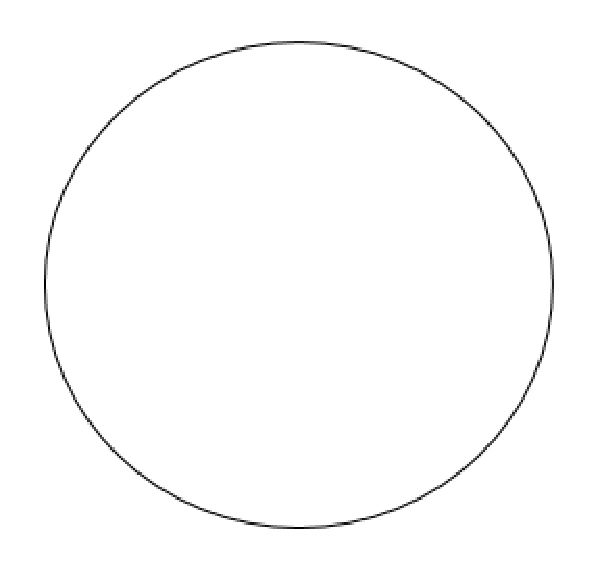
\includegraphics[scale=0.6]{Figures/HomoCWlindro1}
 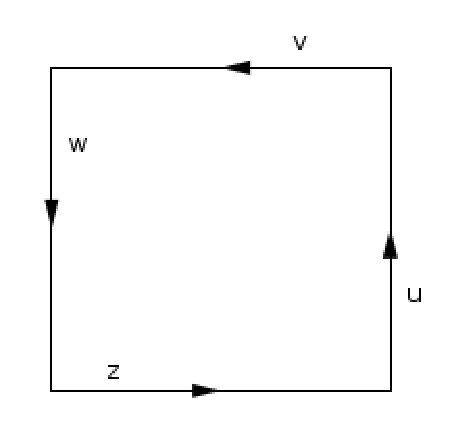
\includegraphics[scale=0.8]{Figures/HomoCWlindro2}
\caption{\label{FigCWlindro1}$S^1$ es homeomorfo al borde de un cuadrado. A cada lado, le asignaremos un 1-símplice singular que lo parametrice.}
\end{figure}

Si $C_i$ es uno de los lados del cuadrado, podemos hallar un 1-símplice singular $\phi_i: \sigma_1 \longrightarrow S^1$ tal que $\phi_i(\sigma_1) \cong C_i$. Por ejemplo, podemos tomar $$\phi_1(t_0,t_1)=\left(\cos\left(\frac{\pi t_0}{4}\right),\sin\left(\frac{\pi t_0}{4}\right)\right)$$ que parametriza el arco de circunferencia correspondiente al primer cuadrante de $\mbR^2$.
\\

Consideremos la cadena $c=u+v-w-z$ descrita en la figura \ref{FigCWlindro1}. Se tiene que $$f_*([c])=f_*([u+v-w-z])=f_*([v])-f_*([z])+f_*([u-w])=f_*([u-w])$$

\begin{figure}[h]
\centering
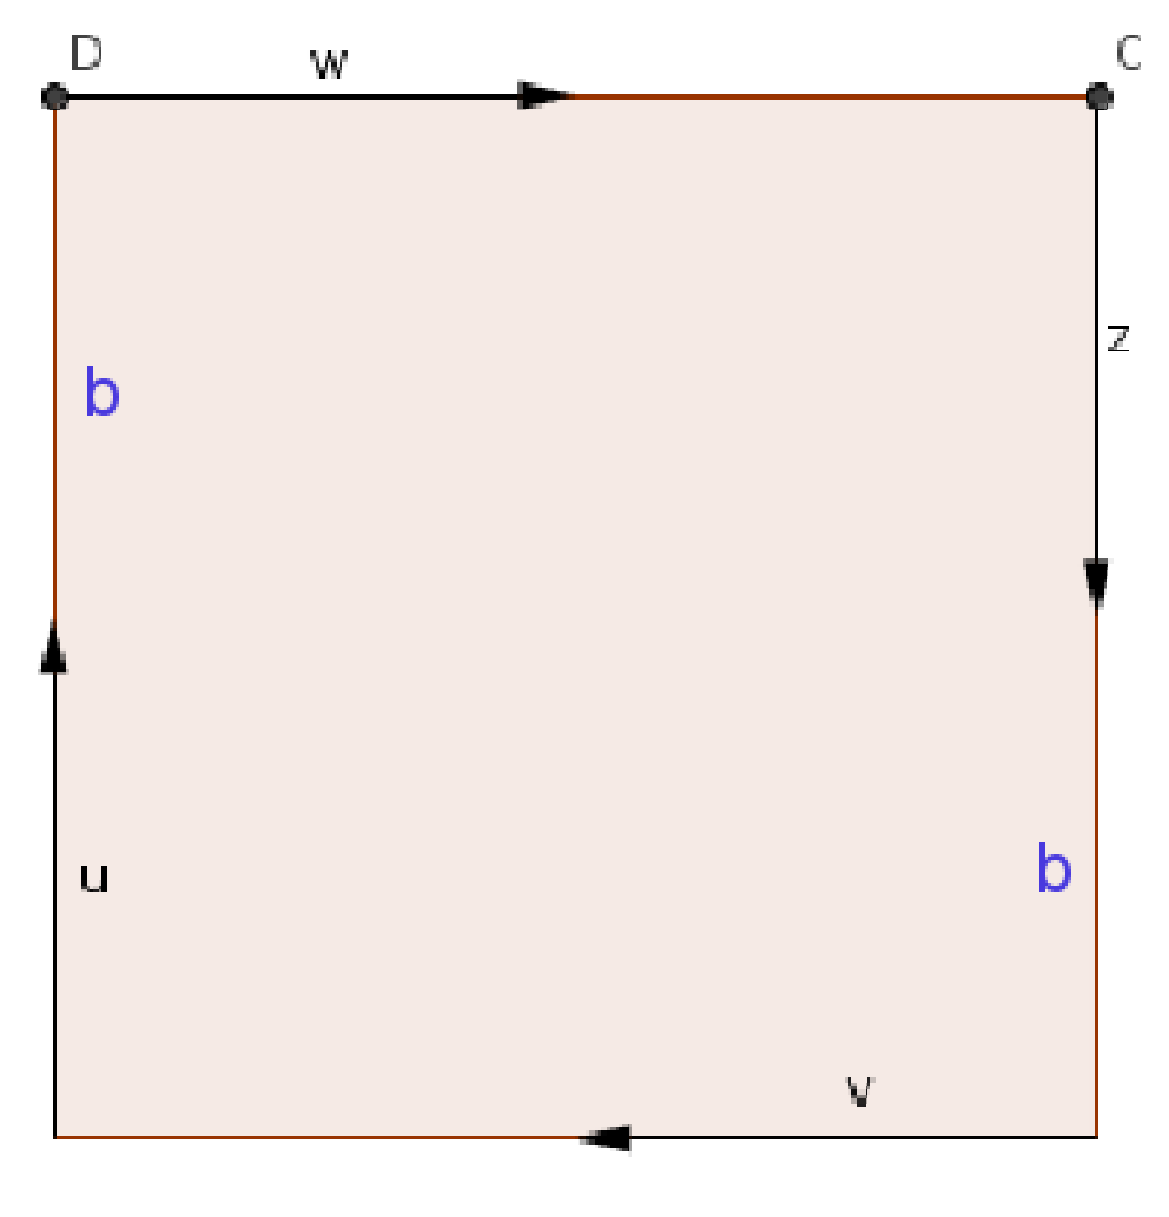
\includegraphics[scale=0.4]{Figures/HomoCWlindro3}
\caption{\label{FigCWlindro2}Los 1-símplices $u$ y $z$ del cuadrado son homólogos y tienen signos opuestos, por lo que se cancelan cuando identificamos los dos lados $b$ del cuadrado.}
\end{figure}

Por tanto, $$\ker f_*=0 \implies \mb{Z} \cong \frac{\tilde{H}_1(S^1)}{\ker f_*} \cong \im f_*$$

De aquí se sigue que \[H_1(8_f) \cong \frac{H_1(8)}{\im f_*}\cong \frac{\mb{Z}^2}{\mb{Z}}=\mb{Z}\] y se tiene la siguiente sucesión exacta corta: \[0 \longrightarrow H_2(8) \xrightarrow{\alpha} H_2(C) \xrightarrow{\beta} \ker f_* \longrightarrow 0\] Como $H_2(8)$ y $\ker f_*$ son ambos cero, se sigue por exactitud que $H_2(C)=0$. Finalmente, para $p > 2$, se tiene que \[H_p(8_f) \cong H_p(8)=0\]

\section{Homología de las superficies compactas}
Según el teorema de clasificación de superficies orientables, tenemos que toda superficie compacta y conexa es homeomorfa a $S^2$, a la suma conexa de $n$ toros o a la suma conexa de $n$ planos proyectivos. Entre otras cosas, eso hace que las componentes conexas de una superficie sean arcoconexas, dado que la arcoconexión es una propiedad topológica.
\\

Si llamamos $S_1,\dots,S_n$ a las componentes conexas de $S$, se tiene que $$H_*(S)\cong \sum^n_{i=1}H_*(S_i)$$ por lo que podemos suponer a efectos de homología que $S$ es arcoconexa.
\\

Por limitaciones de tiempo, nos restringiremos al caso de las superficies orientables, que es más breve.

\subsection{Homología del toro (otro método)}
Como vimos en el ejemplo 7.2, $T_1$ admite una estructura de CW-complejo con una única célula de dimensión 2, por lo que existe una aplicación continua $f: S^1 \longrightarrow 8$ tal que \[T_1\cong 8\cup_f D^2 \implies H_p(T_1)\cong H_p(8)=0 \quad \forall p\neq1,2\]

Vamos a estudiar la aplicación $f_*: \tilde{H}_1(S^1) \longrightarrow H_1(8)$ para poder aplicar la proposición \ref{HomoCW}: sea $\alpha$ el generador de $\tilde{H}_1(S^1)$ y \[c=u-v+w-z\] un representante de la clase $\alpha$, construido como se indica en la figura \ref{ToroCW}.

\begin{figure}[h]
\centering
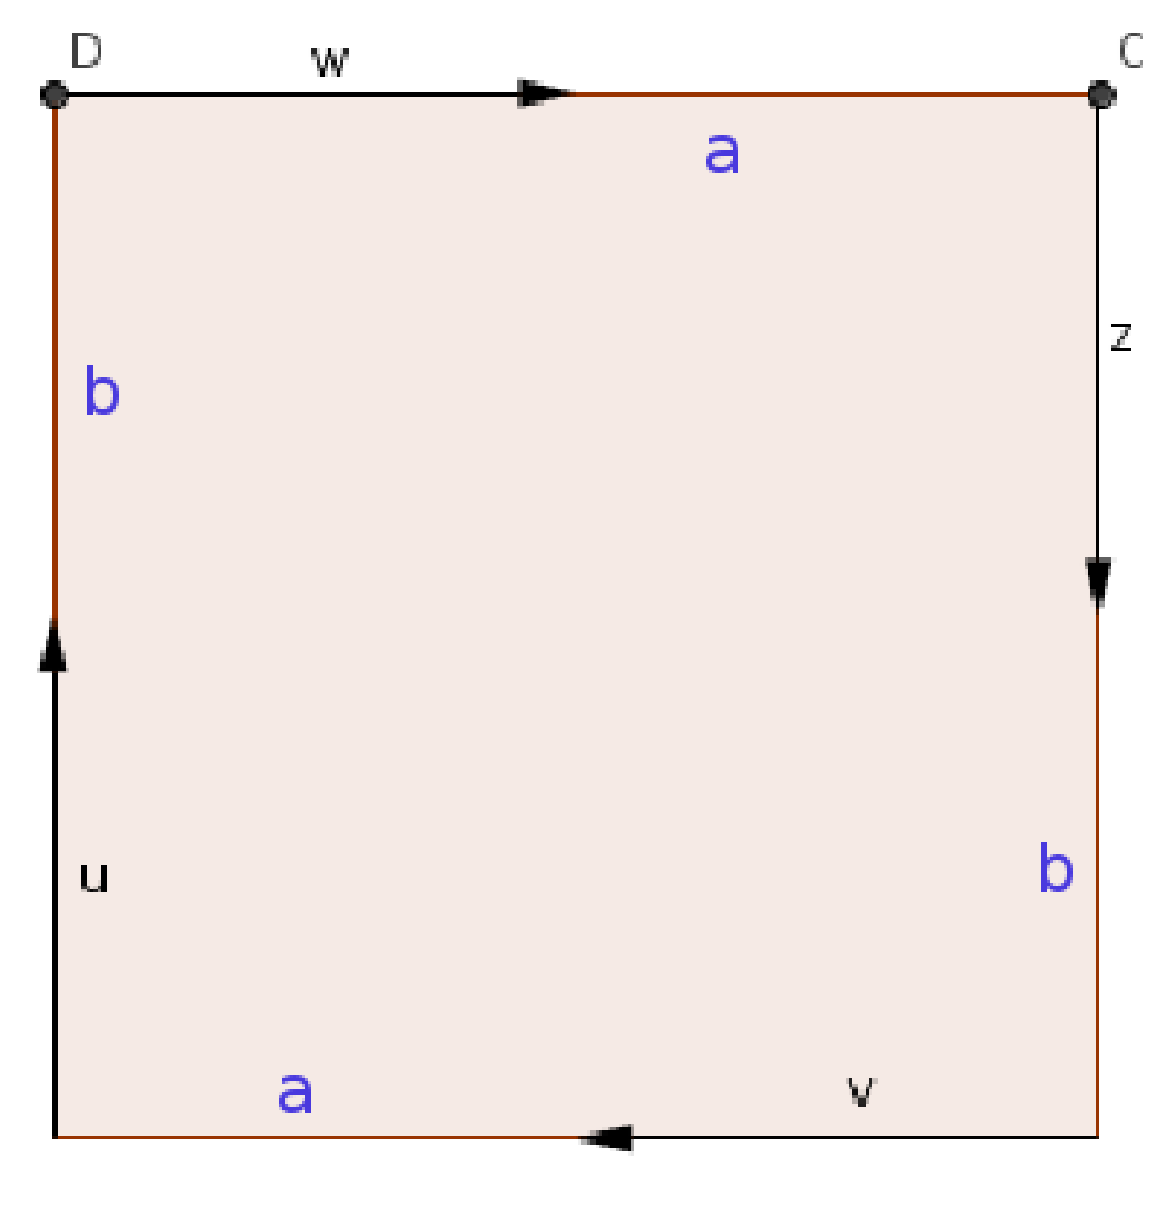
\includegraphics[scale=0.4]{Figures/ToroCW}
\caption{\label{ToroCW}Los lados nombrados como $a$ se identifican entre sí. Lo mismo se aplica a los lados nombrados como $b$.}
\end{figure}

Se tiene que $[f_\#(u)]=[f_\#(z)]$ y $[f_\#(v)]=[f_\#(w)]$, por lo que $$f_*([c])=f_*([u])-f_*([z])+f_*([w])-f_*([v])=0$$ De aquí se deduce que $\ker f_*\cong \mb{Z}$ y que \[\im f_*=0 \implies H_1(T_1)\cong \frac{H_1(8)}{\im f_*}\cong \mb{Z}^2\]

Sólo queda hallar el grupo de orden 2: \[0 \longrightarrow H_2(8) \longrightarrow H_2(T_1) \xrightarrow{\beta} \ker f_* \longrightarrow 0\] Dado que $H_2(8)=0$, se tiene por exactitud que $\beta$ es un isomorfismo, por lo que \[H_2(T_1) \cong \ker f_* \cong \mb{Z}\]

De esta forma, llegamos al mismo resultado con menos operaciones:
\[\tilde{H}_n(T_1)=
\begin{cases}
\mb{Z}^2	&\mbox{ si }n =1\\
\mb{Z}		&\mbox{ si }n =2\\
0     &\mbox{ si no}
\end{cases}\]

\subsection{Homología del bitoro}
El bitoro se define como la suma conexa de dos toros, por lo que el bitoro llano (su representación plana) se define como la suma conexa de dos toros llanos. Podemos ver el bitoro llano en la figura \ref{Bitoro}.
\\ 

\begin{figure}[h]
\centering
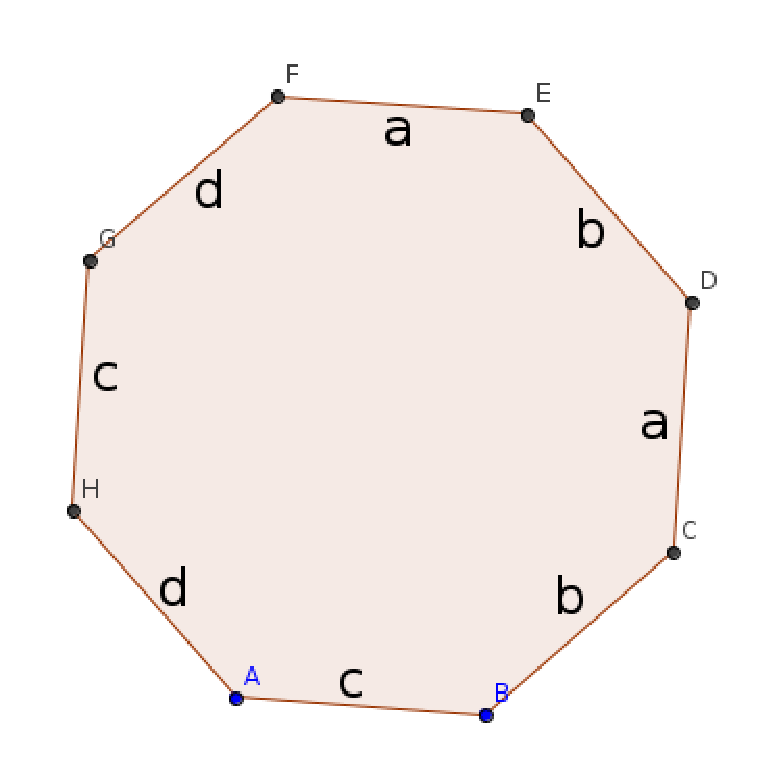
\includegraphics[scale=0.7]{Figures/Bitoro}
\caption{\label{Bitoro} Representación plana del bitoro; los lados etiquetados con la misma letra se identifican entre sí. El subonjunto formado por los lados identificados del octógono forman una rosa de pétalos $a$, $b$, $c$ y $d$.}
\end{figure}

Dado que el octógono es homeomorfo a $D^2$, existe una aplicación continua $f: S^1 \longrightarrow B_4$ tal que \[T_2 \cong B_4 \cup_f D^2\] por lo que el bitoro admite una estructura de CW-complejo.
\\

Vamos a estudiar la aplicación $$f_*: \tilde{H}_1(S^1) \longrightarrow H_1(B_4)$$ Si $\alpha$ es el generador de $\tilde{H}_1(S^1)$, podemos hallar un representante $c$ de $\alpha$ escrito en la forma $$c=u+v+w+z-i-j-k-l$$ (ver figura \ref{BitoroCW}). Al igual que pasaba en el toro, se tiene que $$f_*([c])=0 \implies \ker f_*=\tilde{H}_1(S^1)\; \land\; \im f_*=0$$ Por tanto, $H_p(T_2)\cong H_p(B_4)=0$ para todo $p > 2$ y $H_1(T_2) \cong H_1(B_4)\cong \mb{Z}^4$. Sólo nos queda calcular el grupo de homología de orden 2: \[0 \longrightarrow H_2(B_4) \longrightarrow H_2(T_2) \xrightarrow{\beta} \ker f_* \longrightarrow 0\] Dado que $H_2(B_4)=0$, se tiene por exactitud que $\beta$ es un isomorfismo, por lo que \[H_2(T_2) \cong \ker f_* \cong \mb{Z}\] 

\begin{figure}[h]
\centering
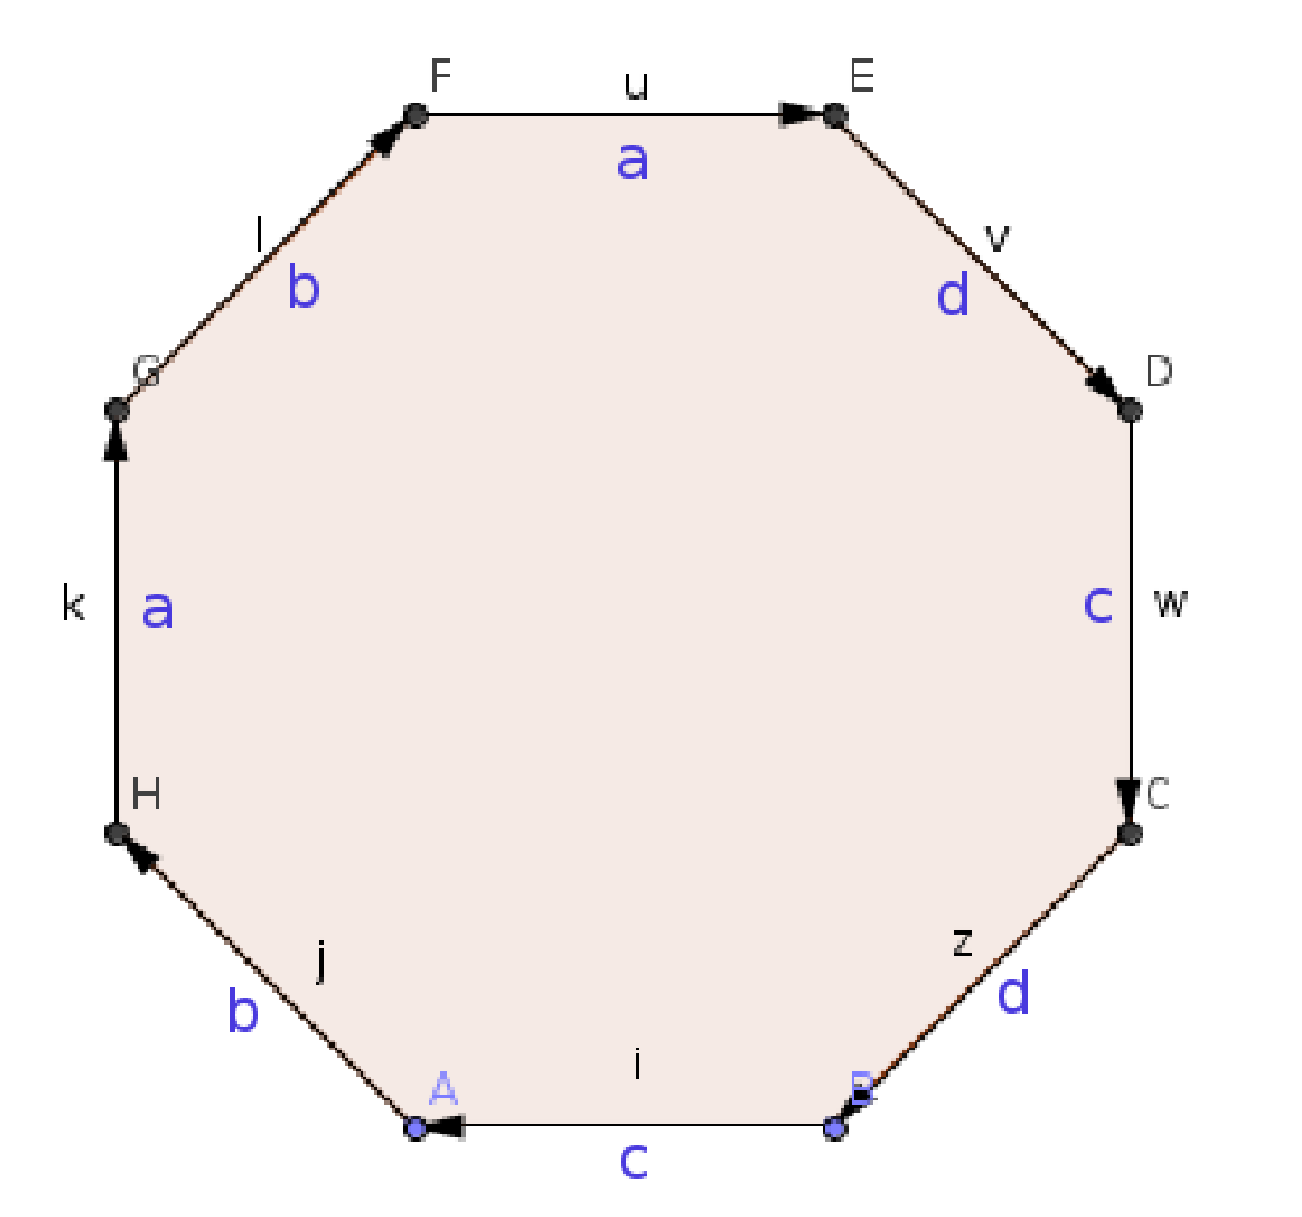
\includegraphics[scale=0.4]{Figures/BitoroCW}
\caption{\label{BitoroCW} Bitoro llano con el generador de $\tilde{H}_1(S^1)$ en el borde.}
\end{figure}

De esta forma, \[\tilde{H}_n(T_2)=
\begin{cases}
\mb{Z}^4	&\mbox{ si }n =1\\
\mb{Z}		&\mbox{ si }n =2\\
0     &\mbox{ si no}
\end{cases}\]

Siguiendo el mismo procedimiento para un $n$ arbitrario, se tiene que $H_1(T_n) \cong H_1(B_{2n})$ y $H_2(T_n)\cong \mb{Z}$.

\begin{teo}\cuadro{Dada una superficie orientable, compacta y conexa $S$, existe un $n > 0$ tal que $$\tilde{H}_q(S)\cong \begin{cases}
\mb{Z}^{2n}	&\mbox{ si }q =1\\
\mb{Z}		&\mbox{ si }q =2\\
0     &\mbox{ si no}
\end{cases}$$ Dicho valor se denomina \textbf{género} de la superficie.}
\end{teo}

Si una superficie tiene género $\lambda$, se tiene que $S \cong T_\lambda$. También se puede definir un género para superficies no orientables; si $S$ es una superficie no orientable de género $\mu$, se tiene que $S \cong P_\lambda$.